% Options for packages loaded elsewhere
\PassOptionsToPackage{unicode}{hyperref}
\PassOptionsToPackage{hyphens}{url}
\PassOptionsToPackage{dvipsnames,svgnames,x11names}{xcolor}
%
\documentclass[
  10pt,
  ignorenonframetext,
]{beamer}
\usepackage{pgfpages}
\setbeamertemplate{caption}[numbered]
\setbeamertemplate{caption label separator}{: }
\setbeamercolor{caption name}{fg=normal text.fg}
\beamertemplatenavigationsymbolsempty
% Prevent slide breaks in the middle of a paragraph
\widowpenalties 1 10000
\raggedbottom
\setbeamertemplate{part page}{
  \centering
  \begin{beamercolorbox}[sep=16pt,center]{part title}
    \usebeamerfont{part title}\insertpart\par
  \end{beamercolorbox}
}
\setbeamertemplate{section page}{
  \centering
  \begin{beamercolorbox}[sep=12pt,center]{part title}
    \usebeamerfont{section title}\insertsection\par
  \end{beamercolorbox}
}
\setbeamertemplate{subsection page}{
  \centering
  \begin{beamercolorbox}[sep=8pt,center]{part title}
    \usebeamerfont{subsection title}\insertsubsection\par
  \end{beamercolorbox}
}
\AtBeginPart{
  \frame{\partpage}
}
\AtBeginSection{
  \ifbibliography
  \else
    \frame{\sectionpage}
  \fi
}
\AtBeginSubsection{
  \frame{\subsectionpage}
}
\usepackage{amsmath,amssymb}
\usepackage{lmodern}
\usepackage{setspace}
\usepackage{iftex}
\ifPDFTeX
  \usepackage[T1]{fontenc}
  \usepackage[utf8]{inputenc}
  \usepackage{textcomp} % provide euro and other symbols
\else % if luatex or xetex
  \usepackage{unicode-math}
  \defaultfontfeatures{Scale=MatchLowercase}
  \defaultfontfeatures[\rmfamily]{Ligatures=TeX,Scale=1}
\fi
% Use upquote if available, for straight quotes in verbatim environments
\IfFileExists{upquote.sty}{\usepackage{upquote}}{}
\IfFileExists{microtype.sty}{% use microtype if available
  \usepackage[]{microtype}
  \UseMicrotypeSet[protrusion]{basicmath} % disable protrusion for tt fonts
}{}
\makeatletter
\@ifundefined{KOMAClassName}{% if non-KOMA class
  \IfFileExists{parskip.sty}{%
    \usepackage{parskip}
  }{% else
    \setlength{\parindent}{0pt}
    \setlength{\parskip}{6pt plus 2pt minus 1pt}}
}{% if KOMA class
  \KOMAoptions{parskip=half}}
\makeatother
\usepackage{xcolor}
\geometry{left = 1cm, right = 0.5cm, top = 0.5cm, bottom = 0.5cm}
\newif\ifbibliography
\usepackage{color}
\usepackage{fancyvrb}
\newcommand{\VerbBar}{|}
\newcommand{\VERB}{\Verb[commandchars=\\\{\}]}
\DefineVerbatimEnvironment{Highlighting}{Verbatim}{commandchars=\\\{\}}
% Add ',fontsize=\small' for more characters per line
\usepackage{framed}
\definecolor{shadecolor}{RGB}{248,248,248}
\newenvironment{Shaded}{\begin{snugshade}}{\end{snugshade}}
\newcommand{\AlertTok}[1]{\textcolor[rgb]{0.94,0.16,0.16}{#1}}
\newcommand{\AnnotationTok}[1]{\textcolor[rgb]{0.56,0.35,0.01}{\textbf{\textit{#1}}}}
\newcommand{\AttributeTok}[1]{\textcolor[rgb]{0.77,0.63,0.00}{#1}}
\newcommand{\BaseNTok}[1]{\textcolor[rgb]{0.00,0.00,0.81}{#1}}
\newcommand{\BuiltInTok}[1]{#1}
\newcommand{\CharTok}[1]{\textcolor[rgb]{0.31,0.60,0.02}{#1}}
\newcommand{\CommentTok}[1]{\textcolor[rgb]{0.56,0.35,0.01}{\textit{#1}}}
\newcommand{\CommentVarTok}[1]{\textcolor[rgb]{0.56,0.35,0.01}{\textbf{\textit{#1}}}}
\newcommand{\ConstantTok}[1]{\textcolor[rgb]{0.00,0.00,0.00}{#1}}
\newcommand{\ControlFlowTok}[1]{\textcolor[rgb]{0.13,0.29,0.53}{\textbf{#1}}}
\newcommand{\DataTypeTok}[1]{\textcolor[rgb]{0.13,0.29,0.53}{#1}}
\newcommand{\DecValTok}[1]{\textcolor[rgb]{0.00,0.00,0.81}{#1}}
\newcommand{\DocumentationTok}[1]{\textcolor[rgb]{0.56,0.35,0.01}{\textbf{\textit{#1}}}}
\newcommand{\ErrorTok}[1]{\textcolor[rgb]{0.64,0.00,0.00}{\textbf{#1}}}
\newcommand{\ExtensionTok}[1]{#1}
\newcommand{\FloatTok}[1]{\textcolor[rgb]{0.00,0.00,0.81}{#1}}
\newcommand{\FunctionTok}[1]{\textcolor[rgb]{0.00,0.00,0.00}{#1}}
\newcommand{\ImportTok}[1]{#1}
\newcommand{\InformationTok}[1]{\textcolor[rgb]{0.56,0.35,0.01}{\textbf{\textit{#1}}}}
\newcommand{\KeywordTok}[1]{\textcolor[rgb]{0.13,0.29,0.53}{\textbf{#1}}}
\newcommand{\NormalTok}[1]{#1}
\newcommand{\OperatorTok}[1]{\textcolor[rgb]{0.81,0.36,0.00}{\textbf{#1}}}
\newcommand{\OtherTok}[1]{\textcolor[rgb]{0.56,0.35,0.01}{#1}}
\newcommand{\PreprocessorTok}[1]{\textcolor[rgb]{0.56,0.35,0.01}{\textit{#1}}}
\newcommand{\RegionMarkerTok}[1]{#1}
\newcommand{\SpecialCharTok}[1]{\textcolor[rgb]{0.00,0.00,0.00}{#1}}
\newcommand{\SpecialStringTok}[1]{\textcolor[rgb]{0.31,0.60,0.02}{#1}}
\newcommand{\StringTok}[1]{\textcolor[rgb]{0.31,0.60,0.02}{#1}}
\newcommand{\VariableTok}[1]{\textcolor[rgb]{0.00,0.00,0.00}{#1}}
\newcommand{\VerbatimStringTok}[1]{\textcolor[rgb]{0.31,0.60,0.02}{#1}}
\newcommand{\WarningTok}[1]{\textcolor[rgb]{0.56,0.35,0.01}{\textbf{\textit{#1}}}}
\setlength{\emergencystretch}{3em} % prevent overfull lines
\providecommand{\tightlist}{%
  \setlength{\itemsep}{0pt}\setlength{\parskip}{0pt}}
\setcounter{secnumdepth}{-\maxdimen} % remove section numbering
\usepackage[absolute,overlay]{textpos}
\usepackage{scalerel,stackengine}
\usepackage{everypage-1x}

\stackMath
\newcommand\reallywidehat[1]{%
\savestack{\tmpbox}{\stretchto{%
  \scaleto{%
    \scalerel*[\widthof{\ensuremath{#1}}]{\kern.1pt\mathchar"0362\kern.1pt}%
    {\rule{0ex}{\textheight}}%WIDTH-LIMITED CIRCUMFLEX
  }{\textheight}% 
}{2.4ex}}%
\stackon[-6.9pt]{#1}{\tmpbox}%
}

\newcommand\MyText[1]{%
  \begin{textblock*}{4.5cm}(0.7\textwidth,6cm)%
    #1
  \end{textblock*}
}
\usepackage{float}
\usepackage{booktabs}
\usepackage[normalem]{ulem}
\useunder{\uline}{\ul}{}
\usepackage{array}
\usepackage{multirow}
\usepackage{mathtools}
\usepackage{xcolor}
\setbeamertemplate{itemize item}{$\diamond$}
\setbeamertemplate{itemize subitem}{\scriptsize$\diamond$}
\setbeamertemplate{navigation symbols}{}
\setbeamertemplate{footline}[page number]
\definecolor{blue}{RGB}{0,114,178}
\definecolor{red}{RGB}{213,94,0}
\definecolor{yellow}{RGB}{240,228,66}
\definecolor{green}{RGB}{0,158,115}
\ifLuaTeX
  \usepackage{selnolig}  % disable illegal ligatures
\fi
\IfFileExists{bookmark.sty}{\usepackage{bookmark}}{\usepackage{hyperref}}
\IfFileExists{xurl.sty}{\usepackage{xurl}}{} % add URL line breaks if available
\urlstyle{same} % disable monospaced font for URLs
\hypersetup{
  pdftitle={Econometrics: Multiple Regression and Applications},
  pdfauthor={Duong Trinh},
  colorlinks=true,
  linkcolor={blue},
  filecolor={Maroon},
  citecolor={Blue},
  urlcolor={Blue},
  pdfcreator={LaTeX via pandoc}}

\title{Econometrics: Multiple Regression and Applications}
\subtitle{ECON4004: LAB 5}
\author{Duong Trinh}
\date{March 6, 2024}
\institute{University of Glasgow}

\begin{document}
\frame{\titlepage}

\setstretch{1.5}
\begin{frame}{Intro}
\protect\hypertarget{intro}{}
\begin{itemize}
\tightlist
\item
  Duong Trinh

  \begin{itemize}
  \tightlist
  \item
    PhD Student in Economics (Bayesian Microeconometrics)
  \item
    Email: \underline{Duong.Trinh@glasgow.ac.uk}
  \end{itemize}
\end{itemize}

\vspace{3mm}

\begin{itemize}
\tightlist
\item
  ECON4004-LB01

  \begin{itemize}
  \tightlist
  \item
    Wednesday 10am -12 pm
  \item
    5 sessions (7-Feb, 14-Feb, 21-Feb, 28-Feb, 6-March)
  \item
    ST ANDREWS:357
  \end{itemize}
\item
  ECON4004-LB02

  \begin{itemize}
  \tightlist
  \item
    Wednesday 12-2 pm
  \item
    5 sessions (7-Feb, 14-Feb, 21-Feb, 28-Feb, 6-March)
  \item
    ST ANDREWS:357
  \end{itemize}
\end{itemize}
\end{frame}

\begin{frame}{Your Attendance \& Lab Feedback}
\protect\hypertarget{your-attendance-lab-feedback}{}
\end{frame}

\begin{frame}{Plan for LAB 5}
\protect\hypertarget{plan-for-lab-5}{}
\begin{itemize}
\tightlist
\item
  Exercise: based on Stock \& Watson, E15.1
\end{itemize}

\vspace{0.8mm}

\begin{itemize}
\tightlist
\item
  We will focus on \emph{``Time Series Regression''}

  \begin{itemize}
  \tightlist
  \item
    Time series data
  \item
    Autocorrelation
  \item
    Autoregressions
  \item
    Forecasting near future values
  \item
    Unit root test
  \end{itemize}
\end{itemize}
\end{frame}

\hypertarget{brief-review}{%
\section{BRIEF REVIEW}\label{brief-review}}

\begin{frame}{Time Series Data - What it looks like\ldots{}}
\protect\hypertarget{time-series-data---what-it-looks-like}{}
\begin{columns}[T]
\begin{column}{.5\textwidth}
\vspace{7mm}

\small

Time series data are data collected on the same observational unit at
multiple time periods (\(t\)).

\vspace{2mm}

\[
\begin{aligned}
&\{y_{t}\}, \\
&t = 1,\ldots, T
\end{aligned}
\]

\vspace{2mm}

Can be of any time frequency - daily, monthly, quarterly, annual,
etc.\footnote[frame]{Typical resource: https://fred.stlouisfed.org/ \\}
\end{column}

\begin{column}{0.48\textwidth}
\begin{flushright}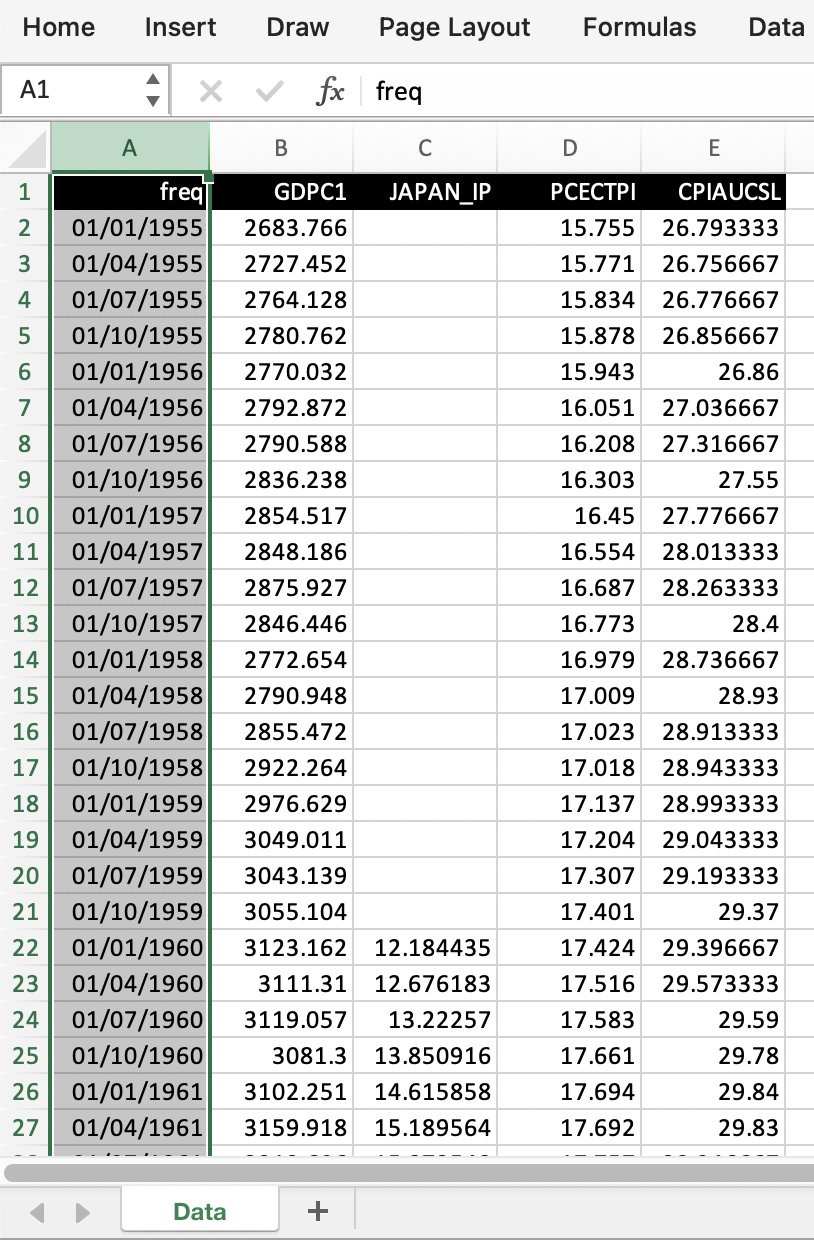
\includegraphics[width=0.9\linewidth]{pictures/TimeSeries-Example} \end{flushright}
\end{column}
\end{columns}
\end{frame}

\begin{frame}{{[}SN{]} Working with dates and times in STATA}
\protect\hypertarget{sn-working-with-dates-and-times-in-stata}{}
\centering Date types in
Stata\footnote[frame]{See guideline at: https://www.stata.com/bookstore/dtguide.pdf \\}
\vspace{0.6mm}

\begin{table}[]
\begin{tabular}{@{}lll@{}}
\toprule
\multicolumn{1}{c}{{\ul \textbf{Date type}}} & \multicolumn{1}{c}{{\ul \textbf{Format}}} & \multicolumn{1}{c}{{\ul \textbf{Unit}}} \\ \midrule
Datetime       & {\textcolor{green}{\texttt{\%tc}}} & Milliseconds since {\textcolor{green}{01jan1960 00:00:00.000}} \\
Daily date     & {\textcolor{green}{\texttt{\%td}}} & Days since {\textcolor{green}{01jan1960}}                     \\
Weekly date    & {\textcolor{green}{\texttt{\%tw}}} & Weeks since {\textcolor{green}{1960w1}}                        \\
Monthly date   & {\textcolor{green}{\texttt{\%tm}}} & Months since {\textcolor{green}{1960m1}}                       \\
Quarterly date & {\textcolor{green}{\texttt{\%tq}}} & Quarters since {\textcolor{green}{1960q1}}                     \\ \bottomrule
\end{tabular}
\end{table}
\end{frame}

\begin{frame}{{[}SN{]} Our Example}
\protect\hypertarget{sn-our-example}{}
\begin{flushleft}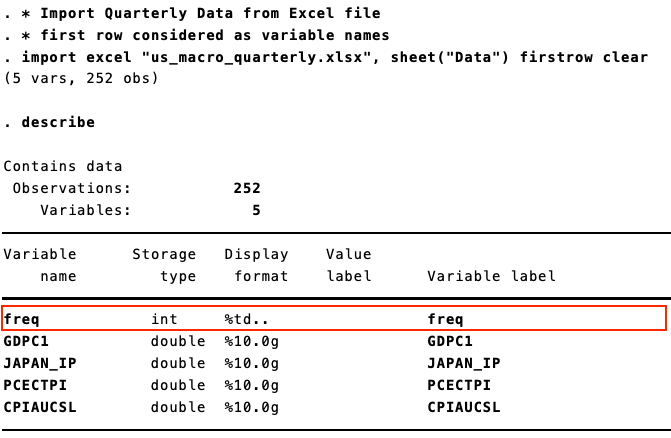
\includegraphics[width=1\linewidth]{pictures/S1-ImportExcelData} \end{flushleft}
\end{frame}

\begin{frame}{{[}SN{]} Creating dates and times in STATA}
\protect\hypertarget{sn-creating-dates-and-times-in-stata}{}
\begin{enumerate}
[(I)]
\tightlist
\item
  Option 1: Building dates and times from
  components.\footnote[frame]{See guideline at: https://www.stata.com/bookstore/dtguide.pdf \\}
\end{enumerate}

\begin{table}[]
\begin{tabular}{@{}llll@{}}
\toprule
\multicolumn{1}{c}{{\ul \textbf{Date type}}} &
  \multicolumn{1}{c}{{\ul \textbf{Format}}} &
  \multicolumn{1}{c}{{\ul \textbf{Pseudofunction}}} &
  \multicolumn{1}{c}{{\ul \textbf{Function}}} \\ \midrule
Daily date     & {\textcolor{green}{\texttt{\%td}}} & td(day-month-year) & mdy(M, D, Y) \\
Weekly date    & {\textcolor{green}{\texttt{\%tw}}} & tw(year-week)      & yw(Y, W)     \\
Monthly date   & {\textcolor{green}{\texttt{\%tm}}} & tm(year-month)     & ym(Y, M)     \\
Quarterly date & {\textcolor{green}{\texttt{\%tq}}} & tq(year-quarter)   & yq(Y, Q)     \\ \bottomrule
\end{tabular}
\end{table}
\end{frame}

\begin{frame}{{[}SN{]} Our Example}
\protect\hypertarget{sn-our-example-1}{}
\begin{flushleft}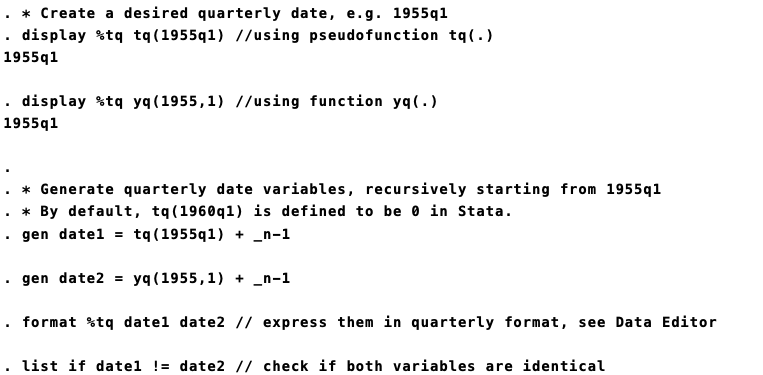
\includegraphics[width=1\linewidth]{pictures/S2-GenDate-Opt1} \end{flushleft}
\end{frame}

\begin{frame}{{[}SN{]} Creating dates and times in STATA}
\protect\hypertarget{sn-creating-dates-and-times-in-stata-1}{}
\begin{enumerate}
[(I)]
\setcounter{enumi}{1}
\tightlist
\item
  Option 2: Converting dates and times from existing
  variables.\footnote[frame]{See guideline at: https://www.stata.com/bookstore/dtguide.pdf \\}
\end{enumerate}

\begin{center}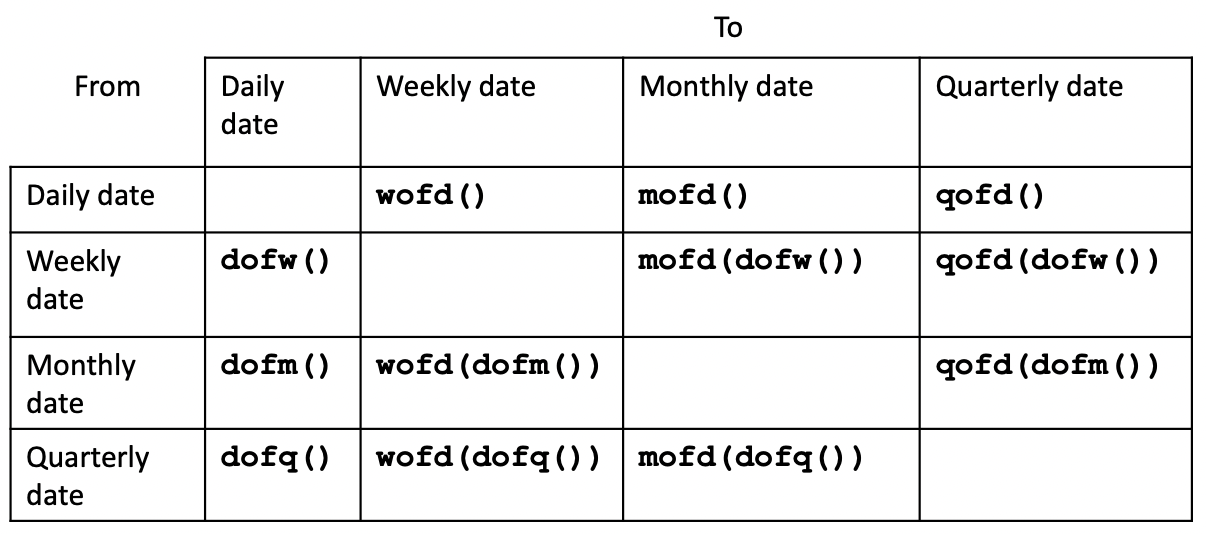
\includegraphics[width=0.9\linewidth]{pictures/ConvertingDates} \end{center}
\end{frame}

\begin{frame}{{[}SN{]} Our Example}
\protect\hypertarget{sn-our-example-2}{}
\begin{flushleft}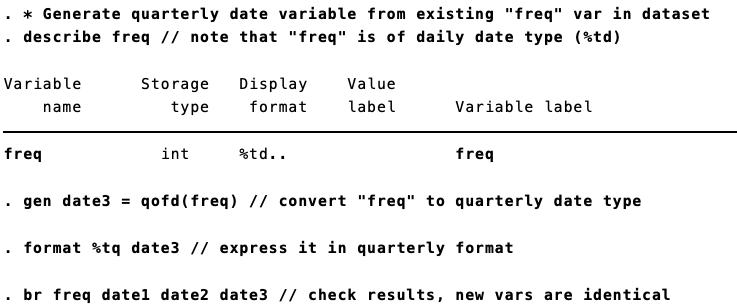
\includegraphics[width=0.9\linewidth]{pictures/S2-GenDate-Opt2} \end{flushleft}

\begin{center}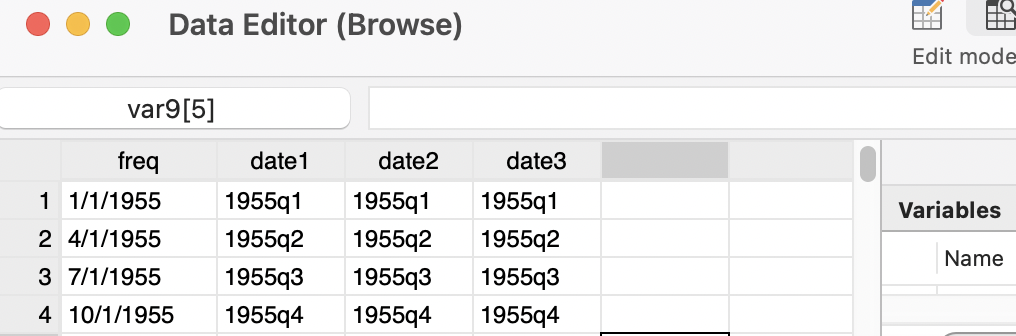
\includegraphics[width=0.7\linewidth]{pictures/S2-GenDate-Compare} \end{center}
\end{frame}

\begin{frame}[fragile]{{[}SN{]} STATA command for Setting Data as Time
Series}
\protect\hypertarget{sn-stata-command-for-setting-data-as-time-series}{}
Once having the date variable in a \emph{date format}, we need to
declare our data as time series to use the time series operators in
Stata.

\small

\begin{Shaded}
\begin{Highlighting}[]
\NormalTok{*}\KeywordTok{tsset}\NormalTok{ datevar}
\CommentTok{//choose suitable \textquotesingle{}datevar\textquotesingle{} in the dataset}
\end{Highlighting}
\end{Shaded}

\begin{flushleft}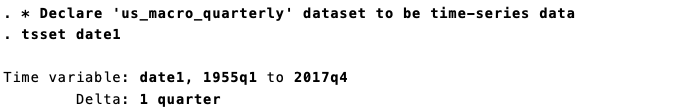
\includegraphics[width=0.9\linewidth]{pictures/S3-DeclareTimeSeries} \end{flushleft}
\end{frame}

\begin{frame}[fragile]{{[}SN{]} STATA command for Visualizing Time
Series Data}
\protect\hypertarget{sn-stata-command-for-visualizing-time-series-data}{}
\small

\begin{Shaded}
\begin{Highlighting}[]
\NormalTok{*[}\KeywordTok{twoway}\NormalTok{] }\KeywordTok{tsline}\NormalTok{ varlist\_of\_inteterest}
\end{Highlighting}
\end{Shaded}

\begin{flushleft}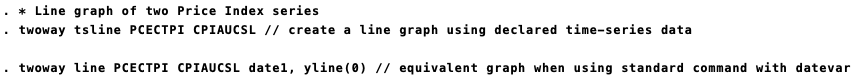
\includegraphics[width=0.9\linewidth]{pictures/S4-LineGraphExample-code} \end{flushleft}

\begin{center}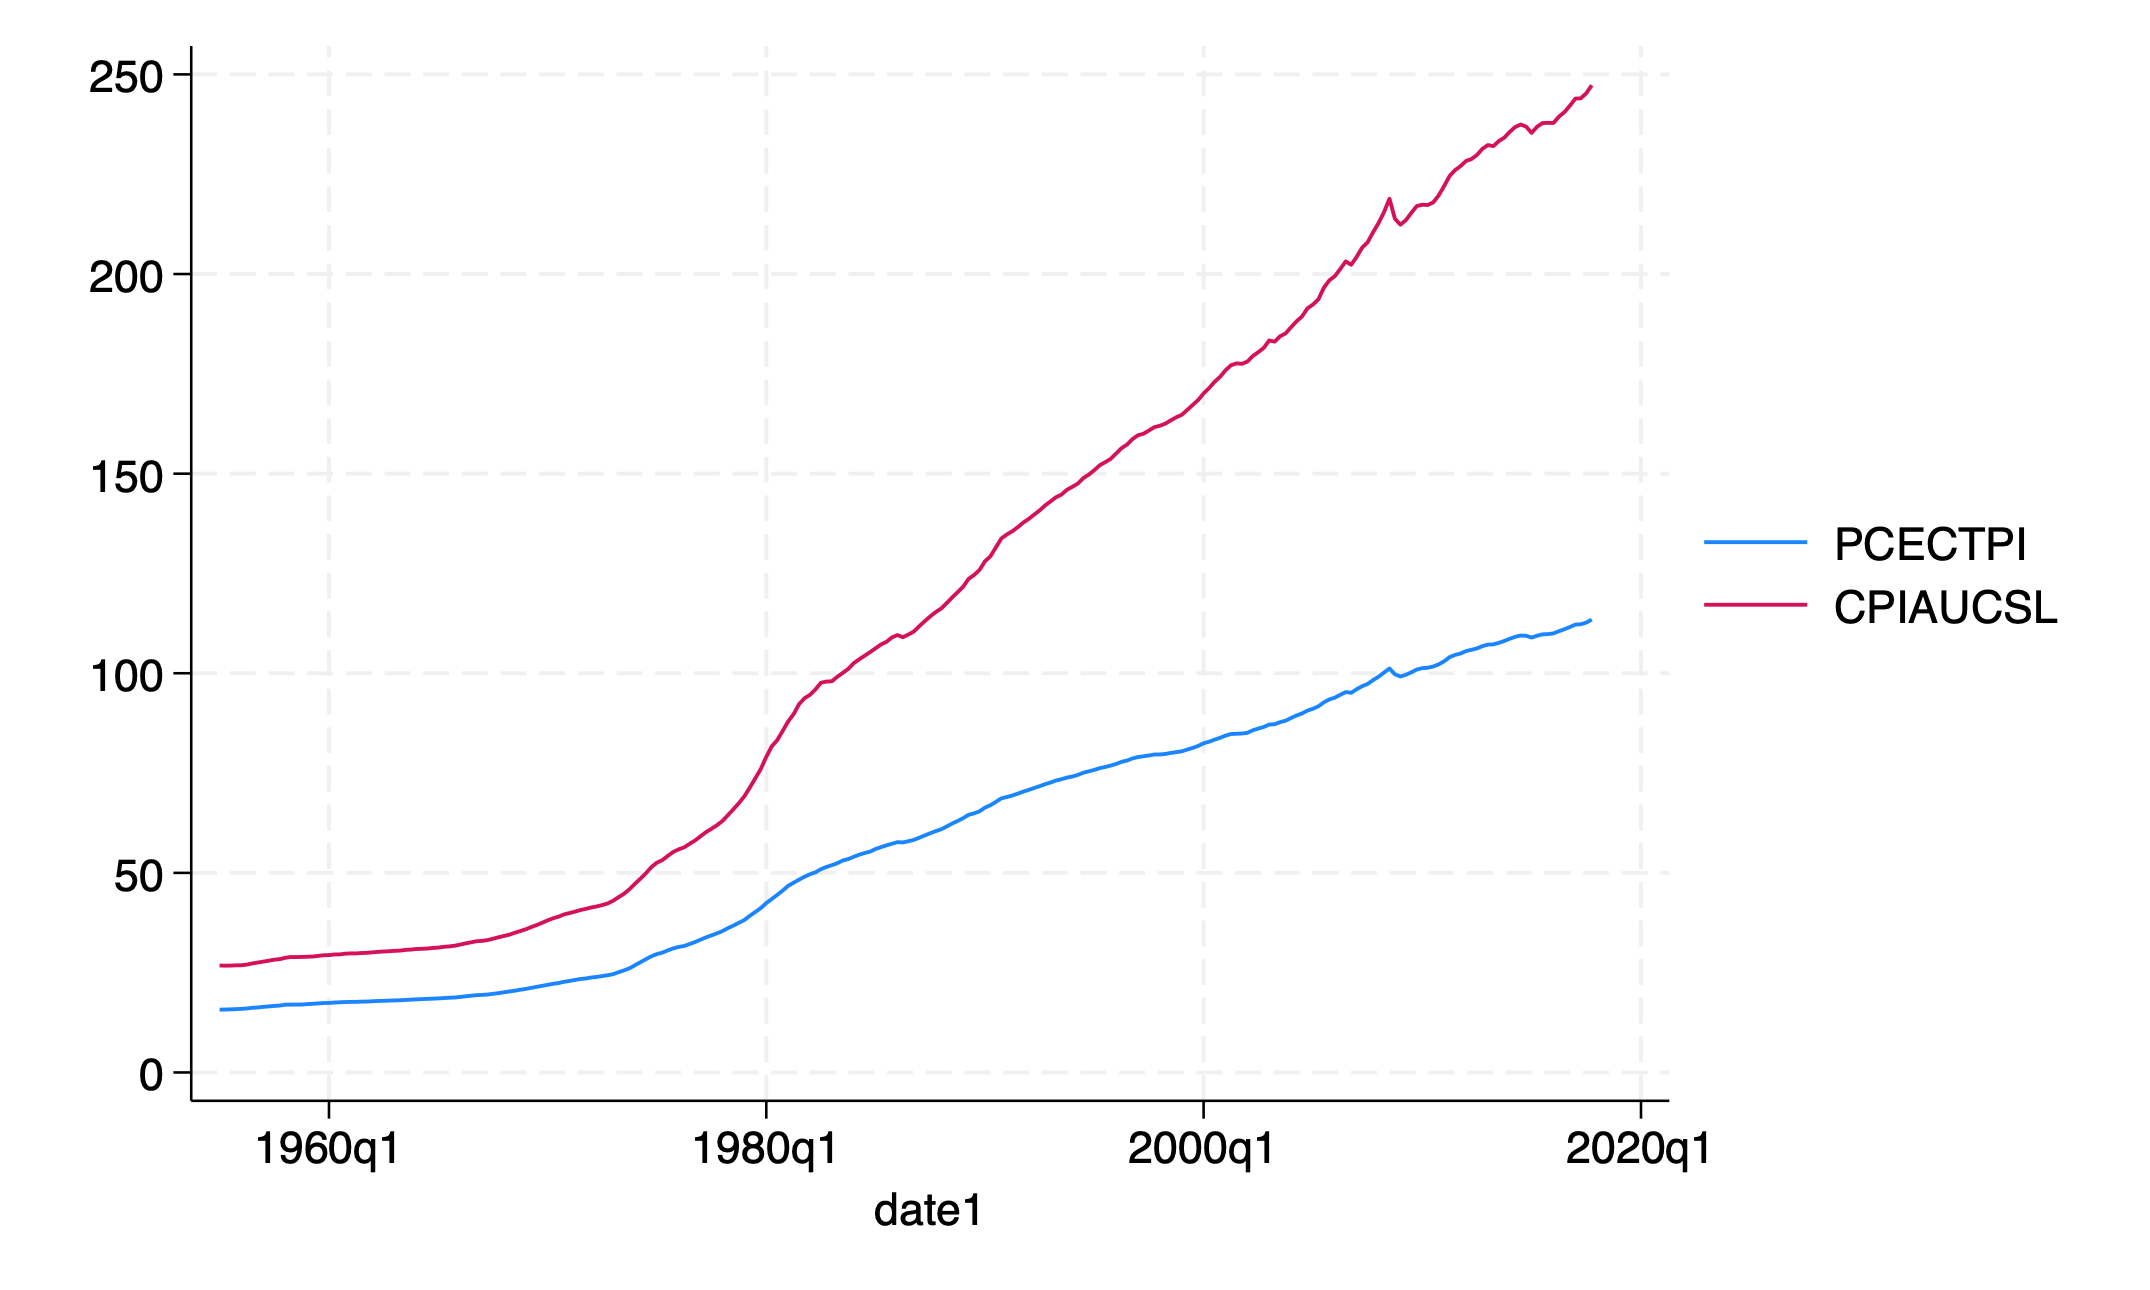
\includegraphics[width=0.7\linewidth]{pictures/S4-LineGraphExample} \end{center}
\end{frame}

\begin{frame}[fragile]{{[}SN{]} Subsetting tin/twithin in STATA}
\protect\hypertarget{sn-subsetting-tintwithin-in-stata}{}
\begin{itemize}
\tightlist
\item
  \texttt{tin} (``times in'', from a to b)
\end{itemize}

\vspace{1mm}

\begin{itemize}
\tightlist
\item
  \texttt{twithin} (``times within'', between a and b, it excludes a and
  b).
\end{itemize}
\end{frame}

\begin{frame}{{[}SN{]} Time‐series operators in STATA}
\protect\hypertarget{sn-timeseries-operators-in-stata}{}
\begin{table}[]
Transforming a time‐series y
\begin{tabular}{lll}
& & \textbf{Stata}\\
\multirow{3}{*}{\textbf{L operator}} & first \textit{lag} $y_{t‐1}$                              & \texttt{L{\color{lightgray}{1}}.y}  \\
                            & 2‐period \textit{lag} $y_{t-2}$                                    & \texttt{L2.y}  \\
                            & 3‐period \textit{lag} $y_{t-3}$                                    & \texttt{L3.y}  \\
                            \\
\multirow{3}{*}{\textbf{D operator}} & first \textit{difference} $\Delta y_t = y_t - y_{t-1}$ & \texttt{D{\color{lightgray}{1}}.y}  \\
                            & double \textit{difference} $\Delta y_t - \Delta y_{t-1}$ & \texttt{D2.y}  \\
                            & triple \textit{difference} $(\Delta y_t - \Delta y_{t-1}) - (\Delta y_{t-1} - \Delta y_{t-2})$ & \texttt{D3.y}  \\
\end{tabular}
\end{table}

\vspace{3mm}

The first difference of the logarithm of \(y_t\) is
\(\Delta \text{ln}(y_t) = \text{ln}(y_t) - \text{ln}(y_{t-1})\) \[
\Delta \text{ln}(y_t) \approx \frac{\text{percentage change of time-series y between } t \text{ and } t-1}{100}
\]
\footnotesize \textcolor{gray}{(!) approximation is most accurate when the percentage change is small.}
\end{frame}

\begin{frame}{Autocorrelation and Autocovariance}
\protect\hypertarget{Autocorr}{}
The covariance between \(y_t\) and its \(j^{\text{th}}\) lag \(y_{t-j}\)
is called \(\qquad \qquad \qquad \qquad\) the \(j^{\text{th}}\)
\emph{autocovariance} of the series \(y_t\)\small \[
{\color{red}{j^{\text{th}} \text{autocovariance}}} \equiv Cov(y_t,y_{t-j})
\]

\vspace{2mm}

\normalsize The correlation between \(y_t\) and its \(j^{\text{th}}\)
lag \(y_{t-j}\) is called \(\qquad \qquad \qquad \qquad\) the
\(j^{\text{th}}\) \emph{autocorrelation coefficient}, aka \emph{serial
correlation coefficient}\small \[
{\color{red}{j^{\text{th}} \text{autocorrelation}}} \equiv \rho_j = \rho_{y_t,y_{t-j}} = \frac{Cov(y_t,y_{t-j})}{\sqrt{Var(y_t)Var(y_{t-j})}} \in[-1,1]
\] \(\color{red}{\rightarrow}\)
\textcolor{red}{Measure how dependent $y_t$ is on its past value $y_{t-j}$.}

\vspace{2mm}

\normalsize Autocorrelations of \(y\) as a function of its lags \(j\) is
known as \(\qquad \qquad \qquad \qquad\) the \emph{autocorrelation
function}.
\end{frame}

\begin{frame}[fragile]{{[}SN{]} Tabulate and Graph Autocorrelations in
STATA}
\protect\hypertarget{sn-tabulate-and-graph-autocorrelations-in-stata}{}
Produce a table of the autocorrelations for a time series \small

\begin{Shaded}
\begin{Highlighting}[]
\NormalTok{*}\KeywordTok{corrgram}\NormalTok{ yvar [, lags(}\KeywordTok{p}\NormalTok{)]}
\CommentTok{// limit the number of computed autocorrelations to p}
\end{Highlighting}
\end{Shaded}

\normalsize

Plot the autocorrelation function for a time series (correlogram) with
pointwise confidence intervals \small

\begin{Shaded}
\begin{Highlighting}[]
\NormalTok{*}\KeywordTok{ac}\NormalTok{ yvar [, lags(}\KeywordTok{p}\NormalTok{)]}
\CommentTok{// limit the number of computed autocorrelations to p}
\end{Highlighting}
\end{Shaded}
\end{frame}

\begin{frame}[fragile]{{[}SN{]} STATA command for Autoregression Model}
\protect\hypertarget{ARmodel}{}
The autoregressive model of order \(p\) - \(AR(p)\) \[
y_t = \beta_0 + \beta_1 y_{t-1} + \beta_2 y_{t-2} + \ldots + \beta_p y_{t-p} + \epsilon_t
\]

To regress \(y_t\) against its own lagged values, run one of the
followings \small

\begin{Shaded}
\begin{Highlighting}[]
\NormalTok{*}\KeywordTok{regress}\NormalTok{ yvar L1.yvar L2.yvar Lp.yvar [, }\KeywordTok{robust}\NormalTok{]}
\end{Highlighting}
\end{Shaded}

\begin{Shaded}
\begin{Highlighting}[]
\NormalTok{*}\KeywordTok{regress}\NormalTok{ yvar L(1/}\KeywordTok{p}\NormalTok{).yvar [, }\KeywordTok{robust}\NormalTok{]}
\CommentTok{//\textquotesingle{}p\textquotesingle{} is the number of lags}
\end{Highlighting}
\end{Shaded}
\end{frame}

\begin{frame}[fragile]{{[}SN{]} Forecasting in STATA}
\protect\hypertarget{sn-forecasting-in-stata}{}
Step1. Expanding the Dataset Before Forecasting

\small

Given a set of time‐series observations, STATA typically records the
dates as running from the first until the last observation.

To forecast a date out‐of‐sample, these dates need to be in the data
set, which requires expanding the dataset to include them.

\begin{Shaded}
\begin{Highlighting}[]
\NormalTok{*}\KeywordTok{tsappend}\NormalTok{, add(}\KeywordTok{k}\NormalTok{)}
\CommentTok{//add \textquotesingle{}k\textquotesingle{} dates to the end of the sample}
\end{Highlighting}
\end{Shaded}

\normalsize

Step2. Point Forecasting Out‐of‐Sample

\small

To create a series of predicted values both in‐sample and out‐of‐sample,
after the \textcolor{blue}{\texttt{regress}} command\small

\begin{Shaded}
\begin{Highlighting}[]
\NormalTok{*}\KeywordTok{predict}\NormalTok{ yvar\_hat [}\KeywordTok{if}\NormalTok{]}
\CommentTok{//use \textquotesingle{}if\textquotesingle{} condition to restrict the predicted values}
\end{Highlighting}
\end{Shaded}
\end{frame}

\begin{frame}{Unit Root Test}
\protect\hypertarget{ADFtest}{}
\begin{itemize}
\item
  Testing for unit roots/stochastic trend is a crucial step in time
  series analysis. The presence of a unit root in a time series
  signifies that the series is non-stationary, which can lead to
  spurious regressions and other potentially serious consequences if no
  further transformation is made.

  \begin{itemize}
  \tightlist
  \item
    \textcolor{red}{$H_0:$ $y_t$ has a unit root ($y_t$ is non-stationary)}.
  \item
    \(H_1:\) \(y_t\) has no unit root (\(y_t\) is stationary).
  \end{itemize}
\item
  The Dickey--Fuller test involves fitting the model \[
  y_t = \beta_0 + \rho y_{t-1} + \delta t + u_t
  \] and test \textcolor{red}{$H_0: \rho = 1$}, or, equivalently, that
  \(y_t\) follows a unit root process.
\item
  To control for serial correlation issue, the augmented Dickey--Fuller
  (ADF) test instead fits \[
  \Delta y_t =  \beta_0 + \delta y_{t-1} + \alpha t + \gamma_1\Delta y_{t-1} + \ldots + \gamma_k\Delta y_{t-k} + \epsilon_t
  \] and test \textcolor{red}{$H_0: \delta = 0$}.
\end{itemize}

\qquad\footnotesize \underline{Note}: Possible restrictions:
\(\beta_0 = 0\) (without drift); \(\alpha =0\) (no trend term).
\end{frame}

\begin{frame}[fragile]{{[}SN{]} ADF Test for Unit Roots in STATA}
\protect\hypertarget{sn-adf-test-for-unit-roots-in-stata}{}
Augmented Dickey--Fuller test using \texttt{tsset} data \small

\begin{Shaded}
\begin{Highlighting}[]
\NormalTok{* }\KeywordTok{dfuller}\NormalTok{ yvar }
\end{Highlighting}
\end{Shaded}

\begin{Shaded}
\begin{Highlighting}[]
\NormalTok{* }\KeywordTok{dfuller}\NormalTok{ yvar, trend}
\CommentTok{// include trend term}
\end{Highlighting}
\end{Shaded}

\begin{Shaded}
\begin{Highlighting}[]
\NormalTok{* }\KeywordTok{dfuller}\NormalTok{ yvar, lags(}\KeywordTok{k}\NormalTok{) }\KeywordTok{regress}
\CommentTok{// include \textquotesingle{}k\textquotesingle{} lagged differences and display the regression table}
\end{Highlighting}
\end{Shaded}
\end{frame}

\hypertarget{excercise-based-on-stock-watson-e15.1}{%
\section{Excercise: based on Stock \& Watson,
E15.1}\label{excercise-based-on-stock-watson-e15.1}}

\begin{frame}[fragile]{Picture the Scenario}
\protect\hypertarget{picture-the-scenario}{}
\begin{itemize}
\tightlist
\item
  \textbf{Objective:} Construct forecasting models for the rate of
  inflation.
\end{itemize}

\vspace{0.8mm}

\begin{itemize}
\tightlist
\item
  \textbf{Dataset:} \texttt{us\_macro\_quaterly.xlsx}.

  \begin{itemize}
  \tightlist
  \item
    contains quarterly data on several macroeconomic series for the US.
  \item
    use the sample period \(1963:Q1-2017:Q4\).(where data before 1963
    may be used, as necessary, as initial values for lags in
    regressions)
  \end{itemize}
\end{itemize}

\vspace{0.8mm}

\begin{itemize}
\tightlist
\item
  \textbf{Key variables:} For each country in each year

  \begin{itemize}
  \tightlist
  \item
    \texttt{PCEPI}: the price index for personal consumption
    expenditures from the U.S. National Income and Product Accounts.
  \end{itemize}
\end{itemize}
\end{frame}

\begin{frame}[fragile]{Questions}
\protect\hypertarget{questions}{}
\begin{block}{(a)}
\protect\hypertarget{a}{}
\begin{enumerate}
[i.]
\item
  Compute the inflation rate,
  \(Infl = 400 \times [ln(PCEPI_t) - ln(PCEPI_{t-1})]\). What are the
  units of \texttt{Infl}?
\item
  Plot the values of \texttt{Infl} from 1963:Q1 through 2017:Q4. Based
  on the plot, do you think that \texttt{Infl} has a stochastic trend?
  Explain.
\end{enumerate}

\vspace{1mm}
\end{block}

\begin{block}{(b) Autocorrelations
\footnotesize\protect\hyperlink{Autocorr}{(\textgreater\textgreater review)}
\normalsize}
\protect\hypertarget{b-autocorrelations-review}{}
\begin{enumerate}
[i.]
\item
  Compute the first four autocorrelations of \(\Delta Infl\).
\item
  Plot the value of \(\Delta Infl\) from 1963:Q1 through 2017:Q4. The
  plot should look choppy or jagged. Explain why this behaviour is
  consistent with the first autocorrelation that you computed in (i.).
\end{enumerate}
\end{block}
\end{frame}

\begin{frame}{Questions}
\protect\hypertarget{questions-1}{}
\begin{block}{(c) Autoregression Model
\footnotesize\protect\hyperlink{ARmodel}{(\textgreater\textgreater review)}
\normalsize}
\protect\hypertarget{c-autoregression-model-review}{}
\begin{enumerate}
[i.]
\tightlist
\item
  Run an OLS regression of \(\Delta Infl_t\) on \(\Delta Infl_{t-1}\).
  Does knowing the change in inflation over the current quarter help
  predict the change in inflation over the next quarter? Explain.
\end{enumerate}

\vspace{0.8mm}

\begin{enumerate}
[i.]
\setcounter{enumi}{1}
\tightlist
\item
  Estimate an \(AR(2)\) model of \(\Delta Infl_t\) . Is the \(AR(2)\)
  model better than the \(AR(1)\) model? Explain.
\end{enumerate}

\vspace{0.8mm}

\begin{enumerate}
[i.]
\setcounter{enumi}{2}
\tightlist
\item
  Use the \(AR(2)\) model to predict the change in inflation from
  2017:Q4 to 2018:Q1 - that is, to predict the value of
  \(\Delta Infl_{2018:Q1}\).
\end{enumerate}
\end{block}
\end{frame}

\begin{frame}{Questions}
\protect\hypertarget{questions-2}{}
\begin{block}{(d) ADF test
\footnotesize\protect\hyperlink{ADFtest}{(\textgreater\textgreater review)}
\normalsize}
\protect\hypertarget{d-adf-test-review}{}
\begin{enumerate}
[i.]
\tightlist
\item
  Use the ADF test for \(AR(p)\) regression \[
  \Delta Y_t = \beta_0 + \delta Y_{t-1} + \gamma_1 \Delta Y_{t-1} +\ldots +\gamma_p \Delta Y_{t-p+1} + u_t
  \] using \(2\) lags of \(\Delta Infl\) (so that \(p = 3\) in the above
  equation) to test for a stochastic trend in \(Infl\).
\end{enumerate}

\vspace{0.8mm}

\begin{enumerate}
[i.]
\setcounter{enumi}{1}
\tightlist
\item
  Is that ADF test based on the above regression preferred to the
  regression including a determinstic trend \[
  \Delta Y_t = \beta_0 + \alpha t + \delta Y_{t-1} + \ldots + \gamma_p \Delta Y_{t-p+1} + u_t 
  \] for testing for a stochastic trend in \(Infl\)? Explain.
\end{enumerate}

\vspace{0.8mm}

\begin{enumerate}
[i.]
\setcounter{enumi}{2}
\tightlist
\item
  Based on the ADF tests carried out, does the AR model for \(Infl\)
  contain a unit root?
\end{enumerate}
\end{block}
\end{frame}

\begin{frame}[fragile]{(a-i) Compute the inflation rate \texttt{Infl}.
What is its unit?}
\protect\hypertarget{Plot-infl-A1}{}
\footnotesize \protect\hyperlink{Plot-infl}{(\textgreater\textgreater stata)}
\normalsize

\[
Infl = 400 \times [ln(PCEPI_t) - ln(PCEPI_{t-1})]
\]

\texttt{Infl} is measured in percentage points at annual rate.
\end{frame}

\begin{frame}{(a-ii) Plot values of \texttt{Infl} from 1963:Q1 through
2017:Q4. Do you think that \texttt{Infl} has a stochastic trend?}
\protect\hypertarget{Plot-infl-A2}{}
\begin{center}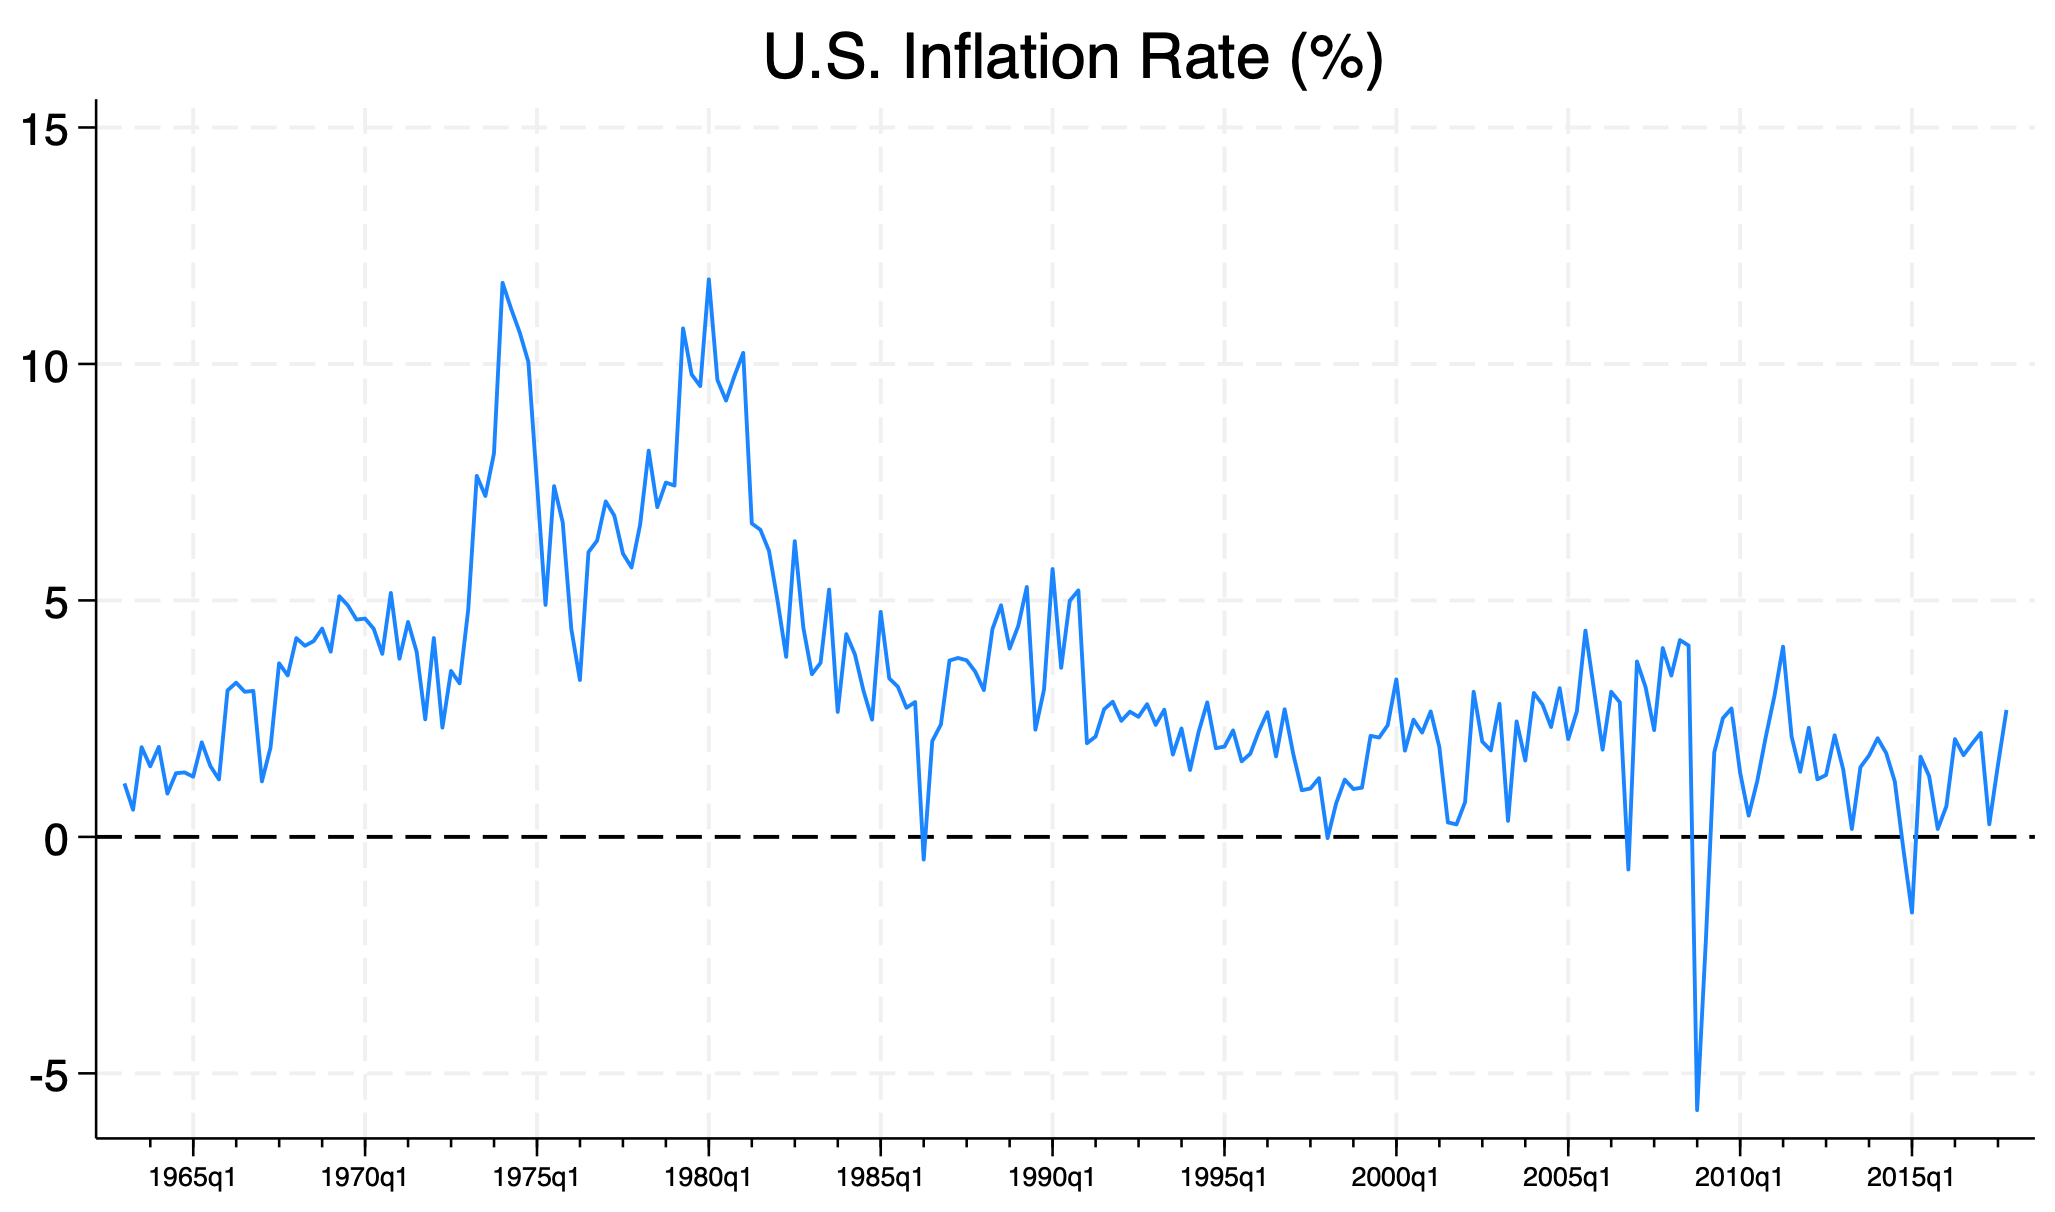
\includegraphics[width=0.85\linewidth]{pictures/Fig1-InflationRate} \end{center}

\footnotesize Inflation increased over the 20-year period 1960-1980,
then declined for a decade and has been reasonably stable since then. It
appears to have a stochastic trend.
\footnotesize \protect\hyperlink{Plot-infl}{(\textgreater\textgreater stata)}
\end{frame}

\begin{frame}[fragile]{(b-i) Compute the first four autocorrelations of
\(\Delta Infl\).}
\protect\hypertarget{b-i-compute-the-first-four-autocorrelations-of-delta-infl.}{}
\small

\begin{Shaded}
\begin{Highlighting}[]
\NormalTok{*}\KeywordTok{corrgram}\NormalTok{ yvar [, lags(}\KeywordTok{p}\NormalTok{)]}
\CommentTok{// limit the number of computed autocorrelations to p}
\end{Highlighting}
\end{Shaded}

\begin{flushleft}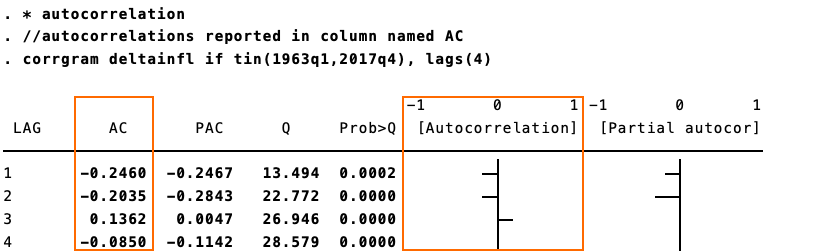
\includegraphics[width=1\linewidth]{pictures/(b-i)corrgram} \end{flushleft}

The first four autocorrelations are (rounded to 2 decimal places):
\(\qquad \qquad \qquad \qquad\) \(-0.25\), \(-0.20\), \(0.14\), and
\(-0.08\).
\end{frame}

\begin{frame}[fragile]{}
\protect\hypertarget{section}{}
\small

\begin{Shaded}
\begin{Highlighting}[]
\NormalTok{*}\KeywordTok{ac}\NormalTok{ yvar [, lags(}\KeywordTok{p}\NormalTok{)]}
\CommentTok{// limit the number of computed autocorrelations to p}
\end{Highlighting}
\end{Shaded}

\begin{flushleft}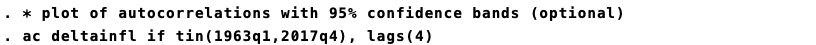
\includegraphics[width=1\linewidth]{pictures/(b-i)ac} \end{flushleft}

\begin{center}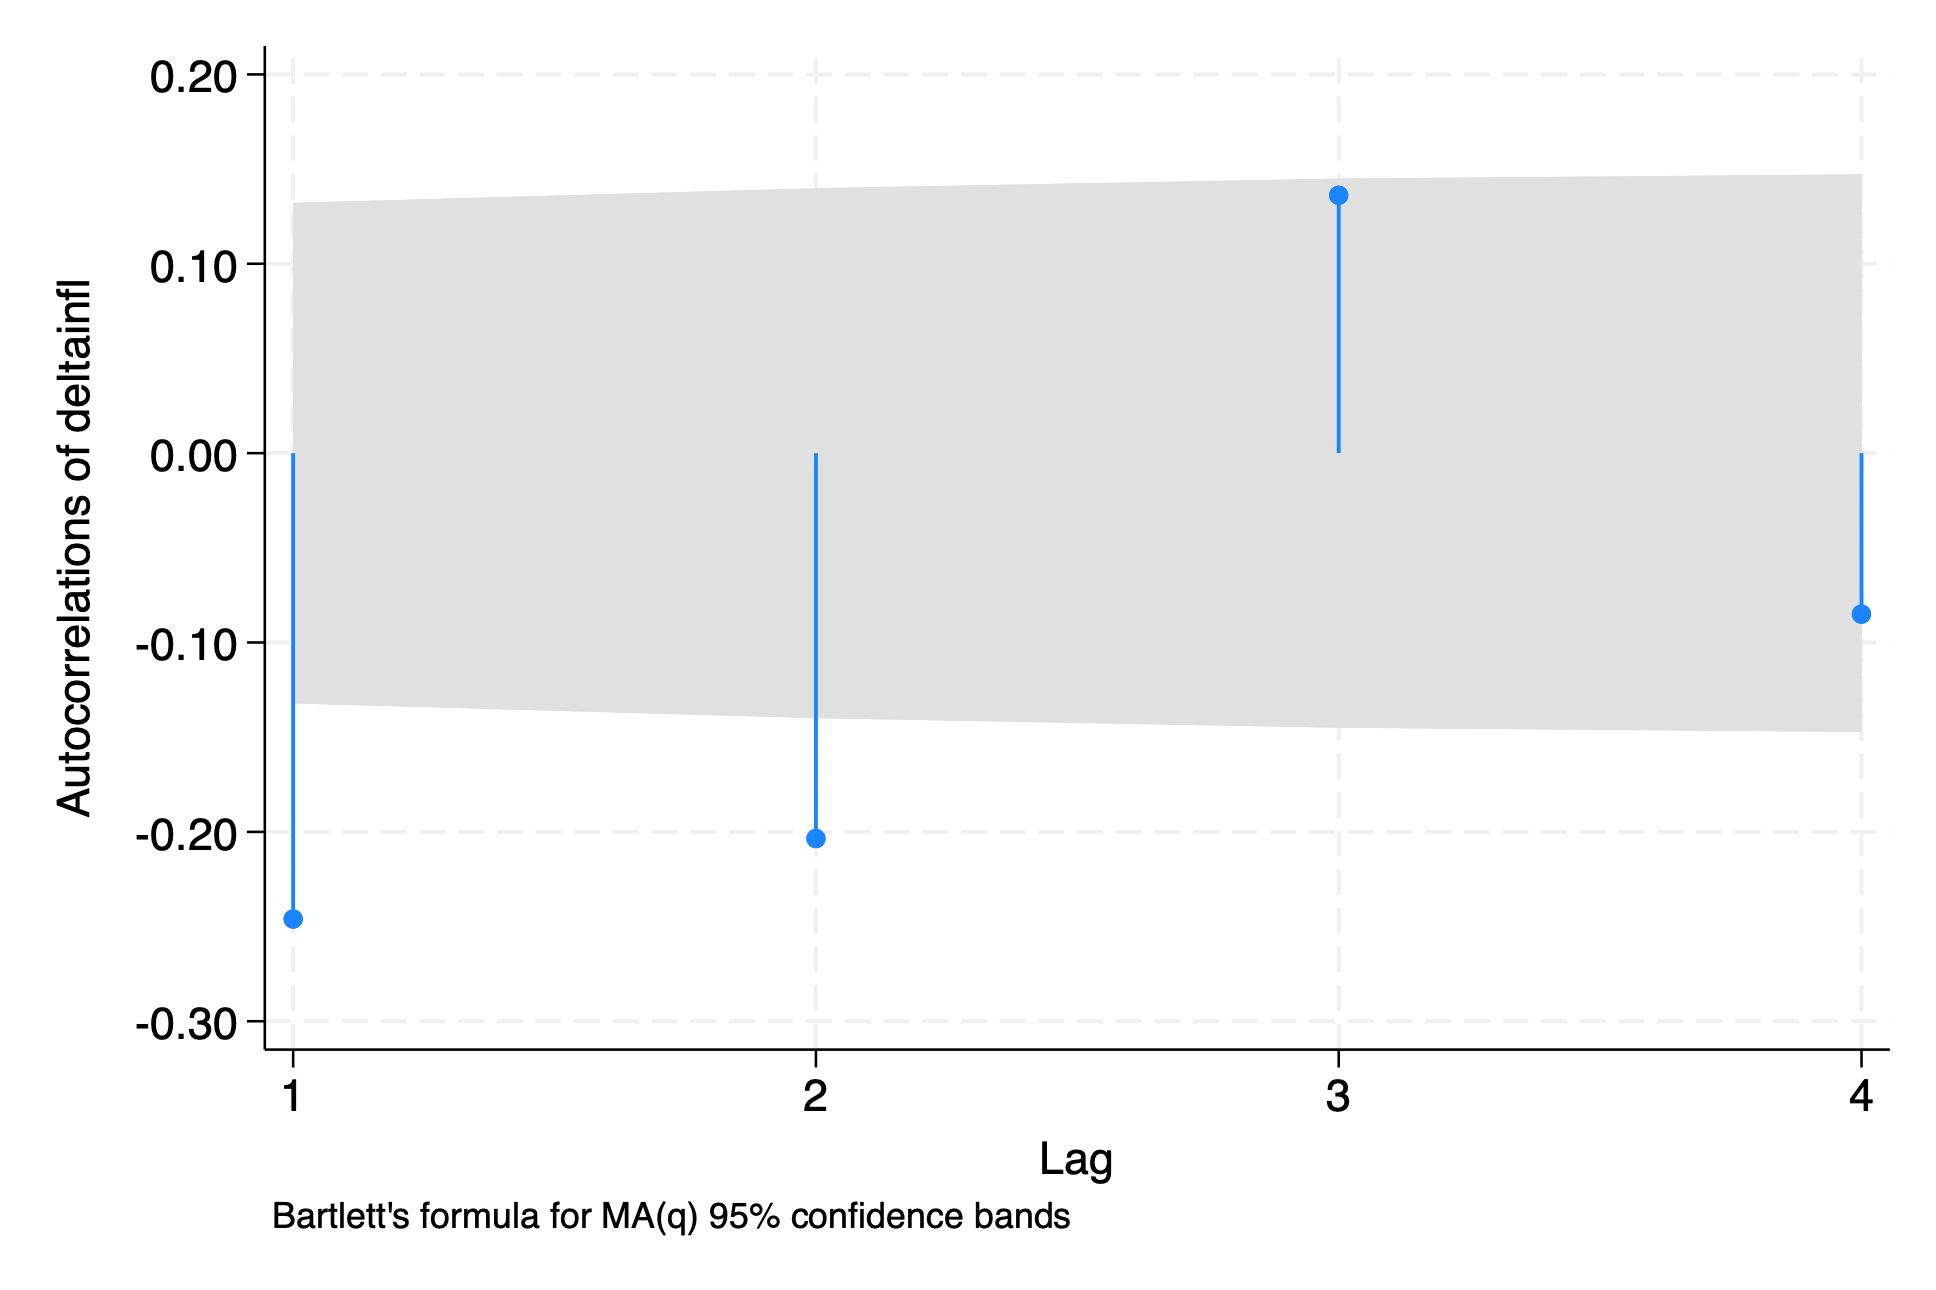
\includegraphics[width=0.7\linewidth]{pictures/AutocorrelationGraph} \end{center}
\end{frame}

\begin{frame}{(b-ii) Plot values of \(\Delta Infl\) from 1963:Q1 through
2017:Q4.}
\protect\hypertarget{Plot-deltainfl-A}{}
\begin{center}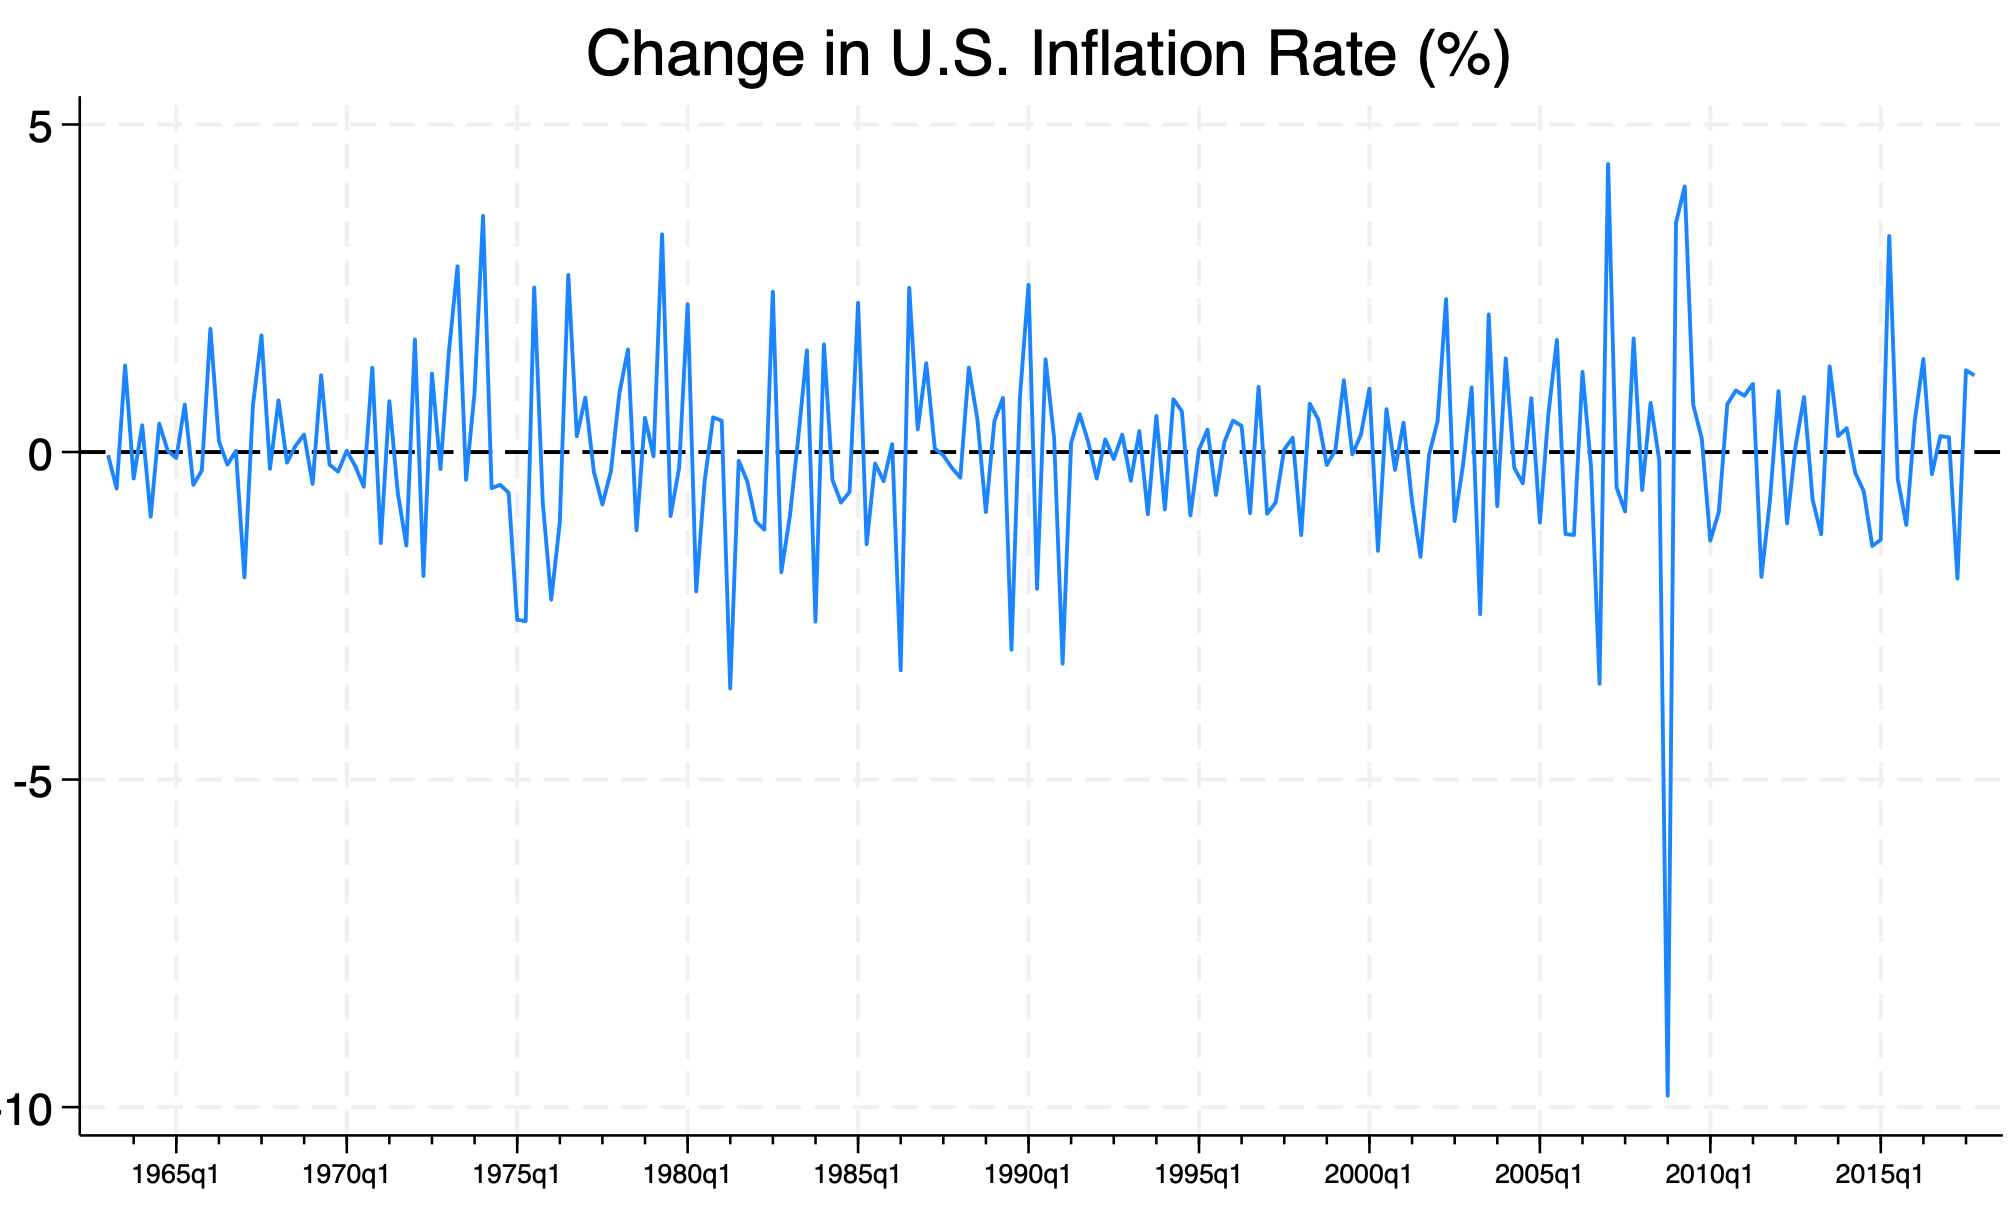
\includegraphics[width=0.85\linewidth]{pictures/Fig2-ChangeInflationRate} \end{center}

\footnotesize The change in inflation is slightly negatively serially
correlated (the first autocorrelation is \(\hat\rho_1 = -0.25\)) so that
values above the mean tend to be followed by values below the mean.
\footnotesize \protect\hyperlink{Plot-deltainfl}{(\textgreater\textgreater stata)}
\end{frame}

\begin{frame}{(c-i) Run an OLS regression of \(\Delta Infl_t\) on
\(\Delta Infl_{t-1}\).}
\protect\hypertarget{c-i-run-an-ols-regression-of-delta-infl_t-on-delta-infl_t-1.}{}
Autoregressive model of order one - AR(1) \[
\Delta Infl_t = \beta_0 + \beta_1 \cdot \Delta Infl_{t-1} + \epsilon_t
\]
\end{frame}

\begin{frame}[fragile]{(c-i) Run an OLS regression of \(\Delta Infl_t\)
on \(\Delta Infl_{t-1}\).}
\protect\hypertarget{c-i-run-an-ols-regression-of-delta-infl_t-on-delta-infl_t-1.-1}{}
\small

\begin{Shaded}
\begin{Highlighting}[]
\NormalTok{*}\KeywordTok{regress}\NormalTok{ yvar L1.yvar [, }\KeywordTok{robust}\NormalTok{]}
\end{Highlighting}
\end{Shaded}

\begin{flushleft}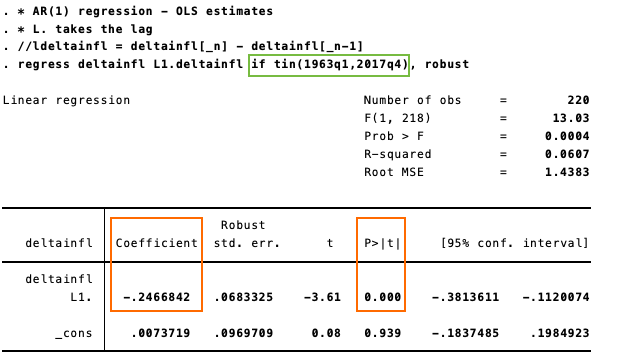
\includegraphics[width=0.9\linewidth]{pictures/(c-i)AR1} \end{flushleft}
\end{frame}

\begin{frame}{(c-i) Run an OLS regression of \(\Delta Infl_t\) on
\(\Delta Infl_{t-1}\). Does knowing the change in inflation over the
current quarter \quad help predict the change in inflation over the next
quarter?}
\protect\hypertarget{AR1-A}{}
Autoregressive model of order one - AR(1) \[
\Delta Infl_t = \beta_0 + \beta_1 \cdot \Delta Infl_{t-1} + \epsilon_t
\]

OLS estimation results
\footnotesize \protect\hyperlink{AR1}{(\textgreater\textgreater stata)}
\normalsize \[
\underset{(se)}{\widehat{\Delta Infl_t}} = \underset{(0.096)}{0.007} -  \underset{(0.068)}{0.247} \cdot \Delta Infl_{t-1}, \qquad R^2=0.061
\]

\begin{itemize}
\tightlist
\item
  The coefficient on lagged inflation is statistically significant, so
  that lagged inflation helps predict current inflation.
\end{itemize}
\end{frame}

\begin{frame}{(c-ii) Estimate an \(AR(2)\) model of \(\Delta Infl_t\).
Is the \(AR(2)\) model better than the \(AR(1)\) model?}
\protect\hypertarget{AR2-A}{}
AR(2) model \[
\Delta Infl_t = \beta_0 + \beta_1 \cdot \Delta Infl_{t-1} + \beta_2 \cdot \Delta Infl_{t-2} +\epsilon_t
\]

\pause

OLS estimation results
\footnotesize \protect\hyperlink{AR2}{(\textgreater\textgreater stata)}
\normalsize \[
\underset{(se)}{\widehat{\Delta Infl_t}} = \underset{(0.093)}{0.006} -  \underset{(0.064)}{0.138} \cdot \Delta Infl_{t-1} - \underset{(0.076)}{0.284} \cdot \Delta Infl_{t-2},\qquad \text{Adj-}R^2=0.128
\]

\begin{itemize}
\tightlist
\item
  The estimated coefficient on \(\Delta Infl_{t-2}\) is statistically
  significant, so the AR(2) model is preferred to the AR(1) model.
\item
  Note also that adjusted R-squared increases from 0.061 in the AR(1)
  model to 0.128 in the AR(2) model, showing better goodness-of-fit.
\end{itemize}
\end{frame}

\begin{frame}{(c-iii) Use the \(AR(2)\) model to predict change in
inflation from 2017:Q4 to 2018:Q1 - that is, value of
\(\Delta Infl_{2018:Q1}\).}
\protect\hypertarget{c-iii-use-the-ar2-model-to-predict-change-in-inflation-from-2017q4-to-2018q1---that-is-value-of-delta-infl_2018q1.}{}
\begin{flushleft}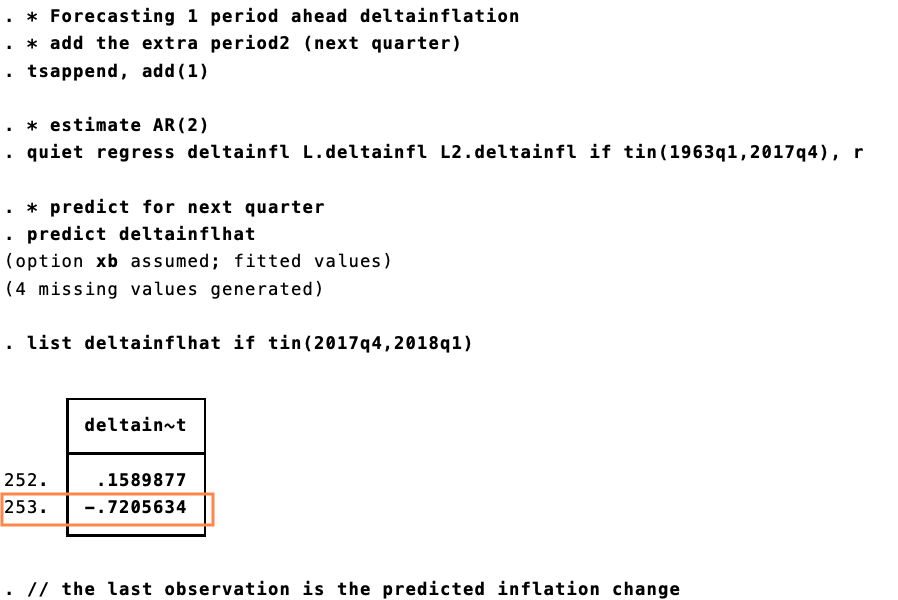
\includegraphics[width=0.9\linewidth]{pictures/(ciii)forecasting} \end{flushleft}
\end{frame}

\begin{frame}{(c-iii) Use the \(AR(2)\) model to predict change in
inflation from 2017:Q4 to 2018:Q1 - that is, value of
\(\Delta Infl_{2018:Q1}\).}
\protect\hypertarget{Plot-forecasting-A}{}
\begin{center}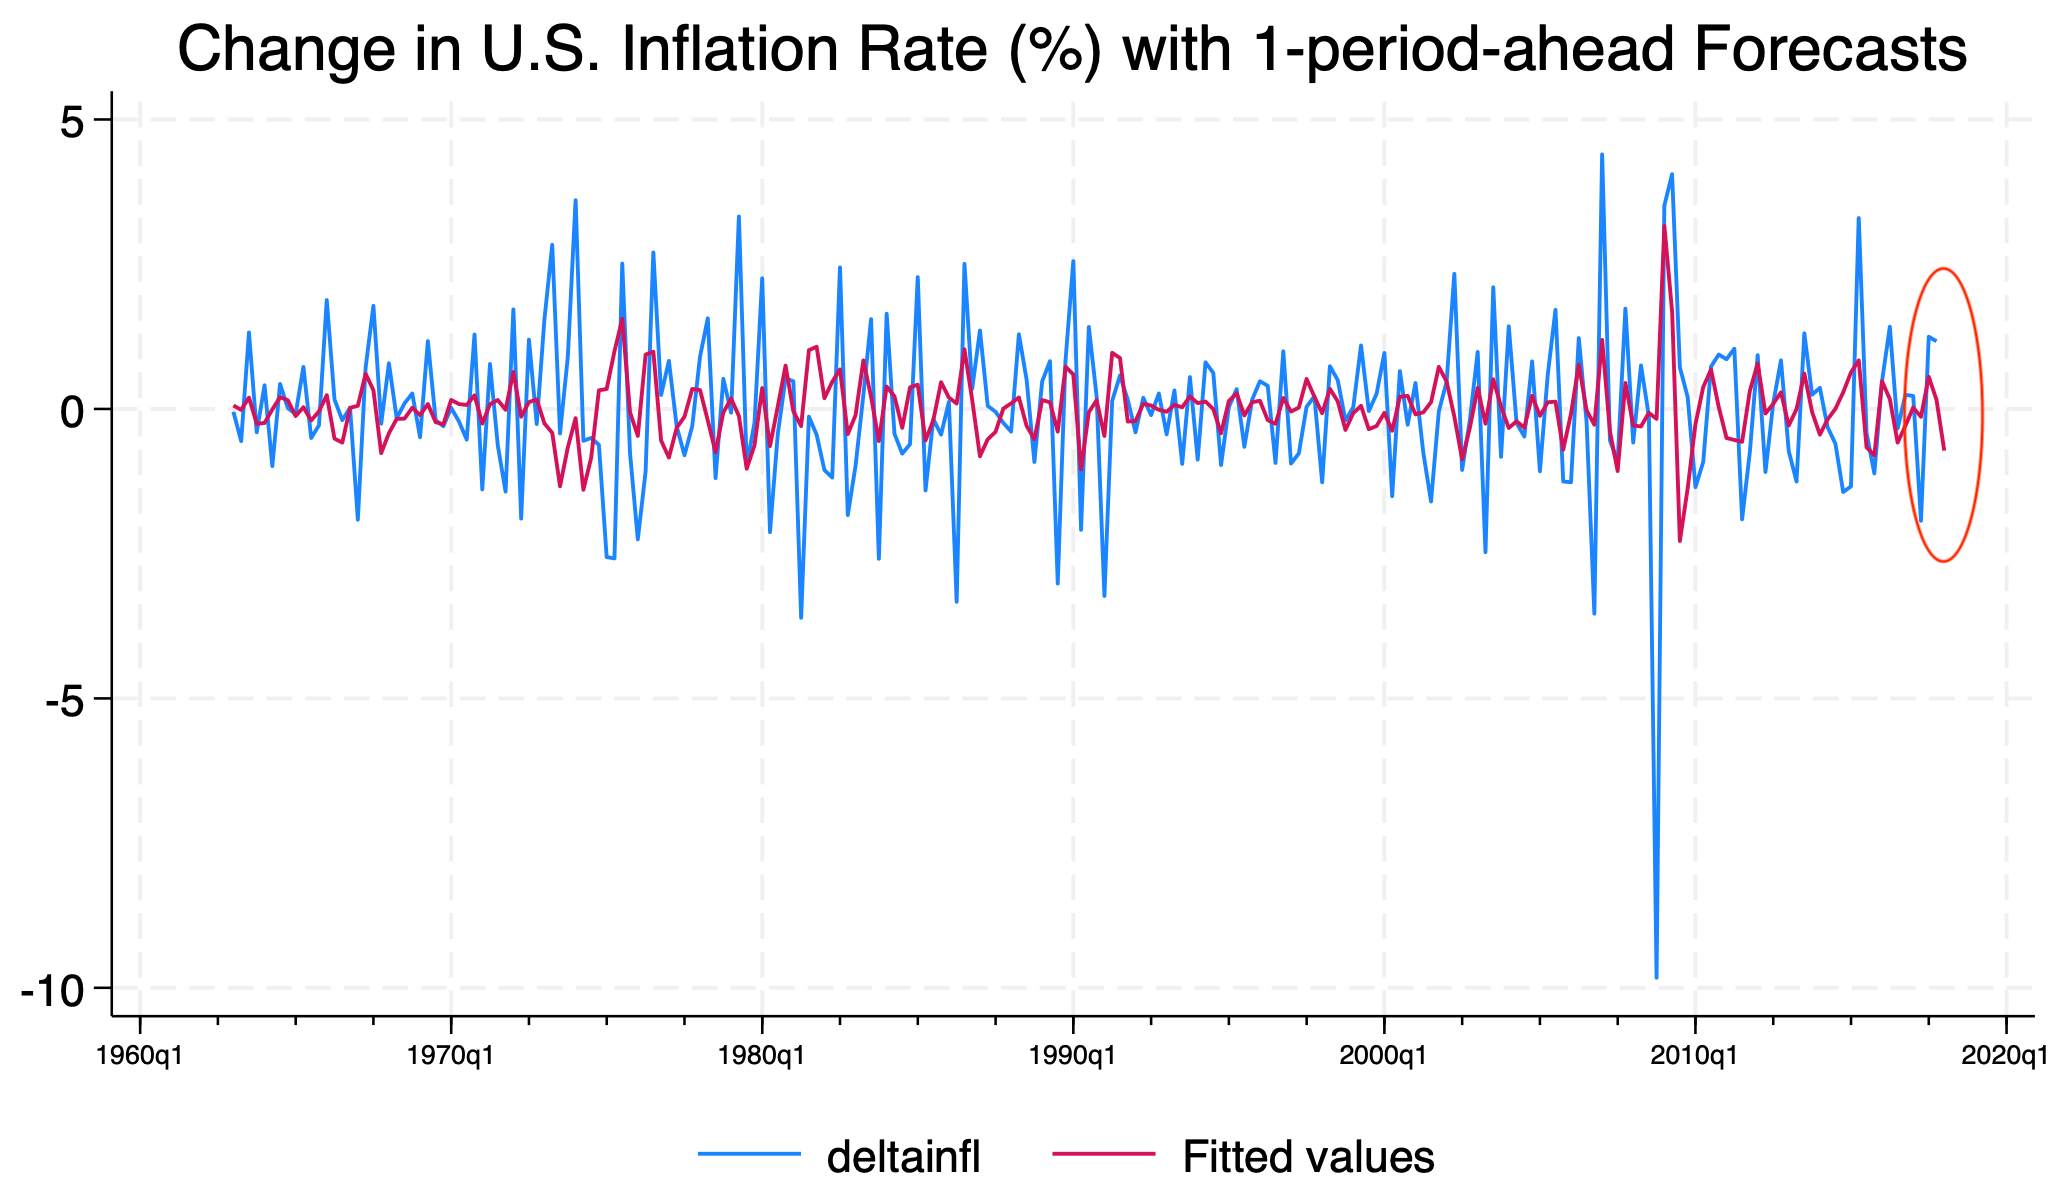
\includegraphics[width=0.85\linewidth]{pictures/Fig3-ForecastChangeInflationRate} \end{center}

\footnotesize The predicted change in inflation from 2017Q4 to 2018Q1 is
\(\mathbf{-0.72}\) (a
drop).\footnotesize \protect\hyperlink{Plot-forecasting}{(\textgreater\textgreater stata)}
\end{frame}

\begin{frame}{(d-i) Use the ADF test for \(AR(p)\) regression using
\(2\) lags of \(\Delta Infl\) (so that \(p = 3\) in the above equation)
to test for a stochastic trend in \(Infl\).}
\protect\hypertarget{d-i-use-the-adf-test-for-arp-regression-using-2-lags-of-delta-infl-so-that-p-3-in-the-above-equation-to-test-for-a-stochastic-trend-in-infl.}{}
\[
\Delta Y_t = \beta_0 + \delta Y_{t-1} + \gamma_1 \Delta Y_{t-1} +\ldots +\gamma_p \Delta Y_{t-p+1} + u_t
\]

\[
\Delta Infl_t = \beta_0 + \delta Infl_{t-1} + \gamma_1 \Delta Infl_{t-1} + \gamma_2 \Delta Infl_{t-2} + u_t
\]
\end{frame}

\begin{frame}[fragile]{}
\protect\hypertarget{section-1}{}
\small

\begin{Shaded}
\begin{Highlighting}[]
\NormalTok{* }\KeywordTok{dfuller}\NormalTok{ yvar, lags(}\KeywordTok{k}\NormalTok{) }\KeywordTok{regress}
\CommentTok{// include \textquotesingle{}k\textquotesingle{} lagged differences and display the regression table}
\end{Highlighting}
\end{Shaded}

\begin{flushleft}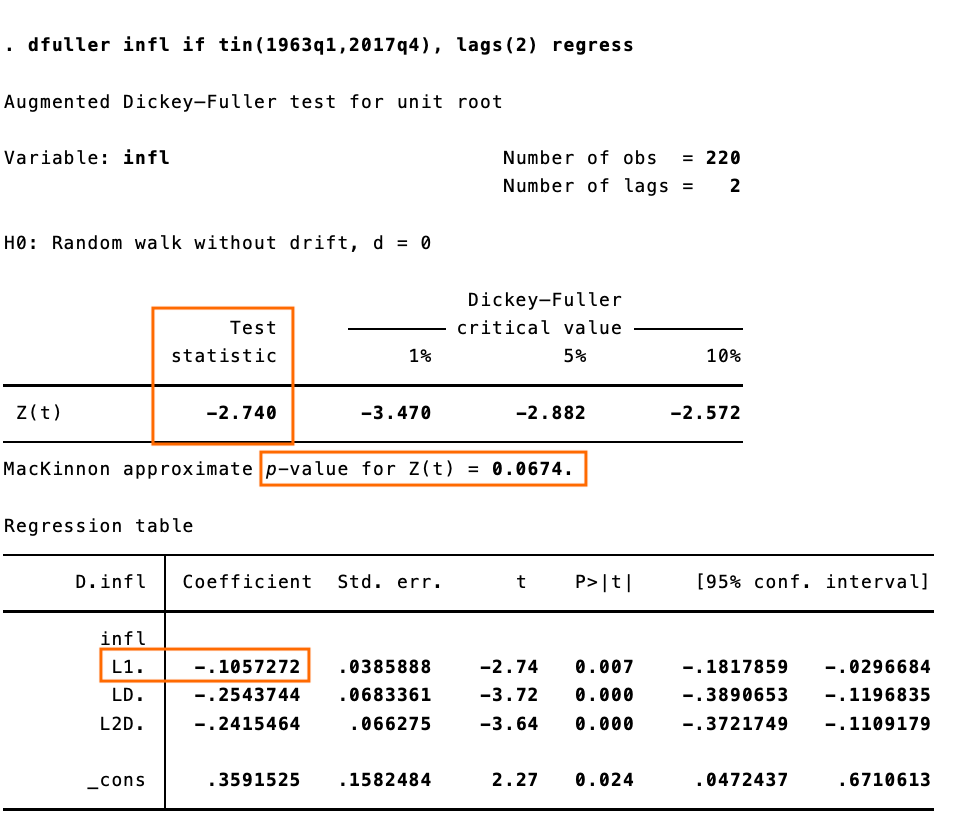
\includegraphics[width=0.7\linewidth]{pictures/(d-i)ADFtest-stochastic} \end{flushleft}
\end{frame}

\begin{frame}{(d-i) Use the ADF test for \(AR(p)\) regression using
\(2\) lags of \(\Delta Infl\) (so that \(p = 3\) in the above equation)
to test for a stochastic trend in \(Infl\).}
\protect\hypertarget{d-i-use-the-adf-test-for-arp-regression-using-2-lags-of-delta-infl-so-that-p-3-in-the-above-equation-to-test-for-a-stochastic-trend-in-infl.-1}{}
The ADF t-statistic is \(-2.74\). The \(10\%\) critical vale is
\(-2.57\) and the \(5\%\) critical value of \(-2.88\); thus the unit
root null hypothesis can be rejected at the \(10\%\) but not the \(5\%\)
significance level.
\end{frame}

\begin{frame}{(d-ii) Is that ADF test based on the above regression
preferred to the regression including a determinstic trend for testing
for a stochastic trend in \(Infl\)?}
\protect\hypertarget{d-ii-is-that-adf-test-based-on-the-above-regression-preferred-to-the-regression-including-a-determinstic-trend-for-testing-for-a-stochastic-trend-in-infl}{}
\[
\Delta Y_t = \beta_0 + \alpha t + \delta Y_{t-1} + \gamma_1\Delta Y_{t-1} + \ldots + \gamma_p \Delta Y_{t-p+1} + u_t 
\]

\[
\Delta Infl_t = \beta_0 + \alpha t + \delta Infl_{t-1} + \gamma_1\Delta Infl_{t-1} + \gamma_2\Delta Infl_{t-2} + u_t 
\]
\end{frame}

\begin{frame}[fragile]{}
\protect\hypertarget{section-2}{}
\small

\begin{Shaded}
\begin{Highlighting}[]
\NormalTok{* }\KeywordTok{dfuller}\NormalTok{ yvar, lags(}\KeywordTok{k}\NormalTok{) trend }\KeywordTok{regress}
\CommentTok{// include \textquotesingle{}k\textquotesingle{} lagged differences and trend term}
\end{Highlighting}
\end{Shaded}

\begin{flushleft}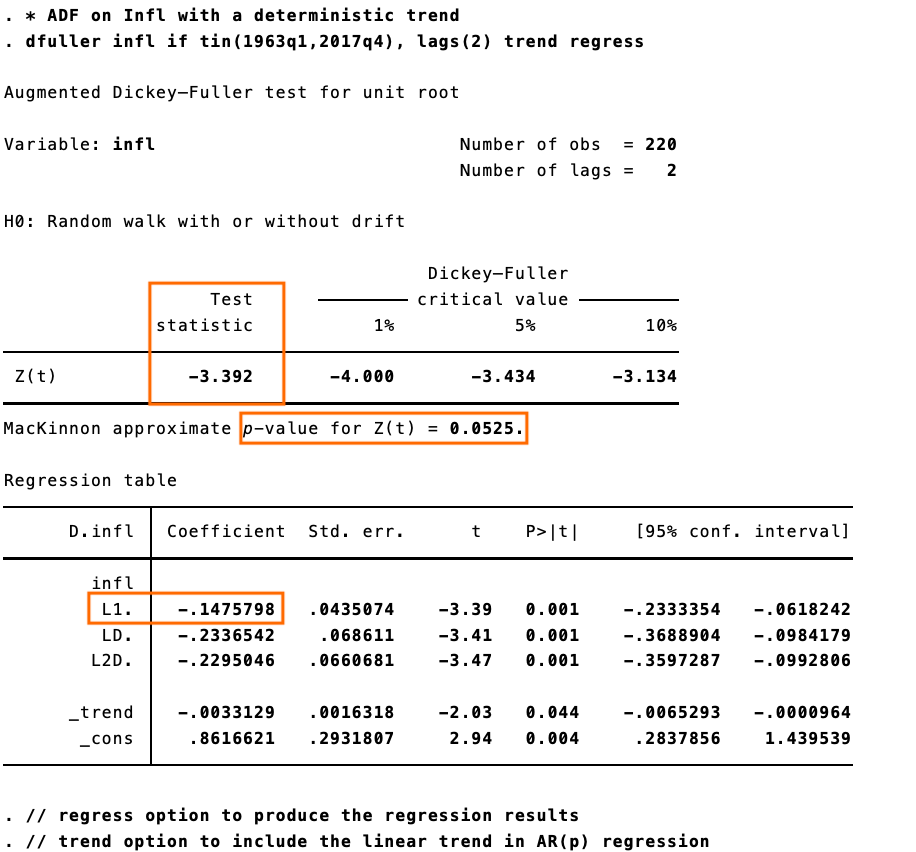
\includegraphics[width=0.7\linewidth]{pictures/(d-ii)ADFtest-deterministic} \end{flushleft}
\end{frame}

\begin{frame}{(d-ii) Is that ADF test based on the above regression
preferred to the regression including a determinstic trend for testing
for a stochastic trend in \(Infl\)?}
\protect\hypertarget{d-ii-is-that-adf-test-based-on-the-above-regression-preferred-to-the-regression-including-a-determinstic-trend-for-testing-for-a-stochastic-trend-in-infl-1}{}
\begin{itemize}
\item
  Based on the t-statistic and the critical values, the results are
  similar to the previous regression.
\item
  The coefficient on trend is quite close to zero so the inflation rate
  does not exhibit a linear trend. Thus, the specification that includes
  an intercept, but no time trend is appropriate.
\end{itemize}
\end{frame}

\begin{frame}{(d-iii) Based on the ADF tests carried out, does the AR
model for \(Infl\) contain a unit root?}
\protect\hypertarget{d-iii-based-on-the-adf-tests-carried-out-does-the-ar-model-for-infl-contain-a-unit-root}{}
\[
\underset{(se)}{\widehat{\Delta Infl_t}} = \underset{(.158)}{.359} -\underset{(.039)}{.106} Infl_{t-1} -\underset{(.068)}{.254} \Delta Infl_{t-1} -\underset{(.066)}{.242}\Delta Infl_{t-2} 
\]

From the results in (d-i), it is clear that inflation contains a unit
root, thereby being highly persistent. The null hypothesis that
\(\delta=0\) or, equivalently, \(\rho = 1.0\) cannot be rejected at the
\(5\%\) significance level.
\end{frame}

\hypertarget{stata-codes-results}{%
\section{STATA CODES \& RESULTS}\label{stata-codes-results}}

\begin{frame}{Q(a-i,ii)
\footnotesize \protect\hyperlink{Plot-infl-A1}{(\textgreater\textgreater back(a-i))}
\protect\hyperlink{Plot-infl-A2}{(\textgreater\textgreater back(a-ii))}
\normalsize }
\protect\hypertarget{Plot-infl}{}
\begin{flushleft}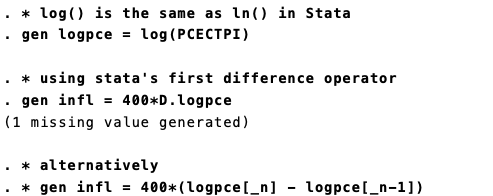
\includegraphics[width=0.65\linewidth]{pictures/(a-i)infl} \end{flushleft}

\vspace{3mm}

\begin{flushleft}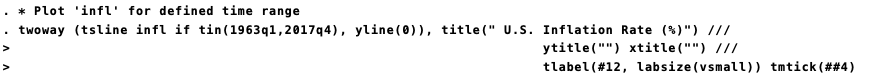
\includegraphics[width=1\linewidth]{pictures/(a-ii)Plot-infl} \end{flushleft}
\end{frame}

\begin{frame}{Q(b-i,ii)
\footnotesize \protect\hyperlink{Plot-infl-A}{(\textgreater\textgreater back(b-ii))}
\normalsize }
\protect\hypertarget{Plot-deltainfl}{}
\begin{flushleft}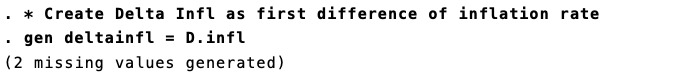
\includegraphics[width=0.8\linewidth]{pictures/(b-i)deltainfl} \end{flushleft}

\vspace{3mm}

\begin{flushleft}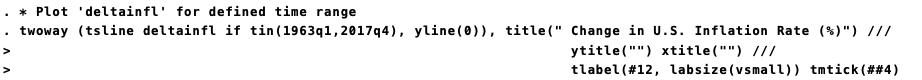
\includegraphics[width=1\linewidth]{pictures/(b-iii)Plot-deltainfl} \end{flushleft}
\end{frame}

\begin{frame}[fragile]{Q(b-i)}
\protect\hypertarget{qb-i}{}
\small

\begin{Shaded}
\begin{Highlighting}[]
\NormalTok{*}\KeywordTok{corrgram}\NormalTok{ yvar [, lags(}\KeywordTok{p}\NormalTok{)]}
\CommentTok{// limit the number of computed autocorrelations to p}
\end{Highlighting}
\end{Shaded}

\begin{flushleft}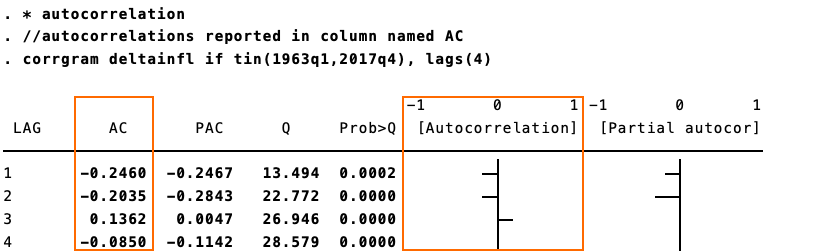
\includegraphics[width=1\linewidth]{pictures/(b-i)corrgram} \end{flushleft}

\small

\begin{Shaded}
\begin{Highlighting}[]
\NormalTok{*}\KeywordTok{ac}\NormalTok{ yvar [, lags(}\KeywordTok{p}\NormalTok{)]}
\CommentTok{// limit the number of computed autocorrelations to p}
\end{Highlighting}
\end{Shaded}

\begin{flushleft}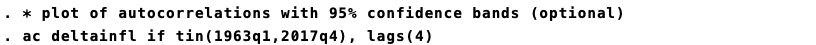
\includegraphics[width=1\linewidth]{pictures/(b-i)ac} \end{flushleft}
\end{frame}

\begin{frame}[fragile]{Q(c-i)
\footnotesize \protect\hyperlink{AR1-A}{(\textgreater\textgreater back(c-i))}
\normalsize }
\protect\hypertarget{AR1}{}
\small

\begin{Shaded}
\begin{Highlighting}[]
\NormalTok{*}\KeywordTok{regress}\NormalTok{ yvar L1.yvar [, }\KeywordTok{robust}\NormalTok{]}
\end{Highlighting}
\end{Shaded}

\begin{flushleft}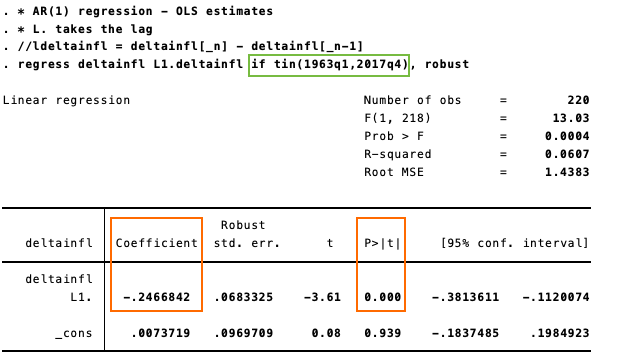
\includegraphics[width=0.9\linewidth]{pictures/(c-i)AR1} \end{flushleft}
\end{frame}

\begin{frame}[fragile]{Q(c-ii)
\footnotesize \protect\hyperlink{AR12-A}{(\textgreater\textgreater back(c-ii))}
\normalsize }
\protect\hypertarget{AR2}{}
\small

\begin{Shaded}
\begin{Highlighting}[]
\NormalTok{*}\KeywordTok{regress}\NormalTok{ yvar L1.yvar L2.yvar [, }\KeywordTok{robust}\NormalTok{]}
\end{Highlighting}
\end{Shaded}

\begin{flushleft}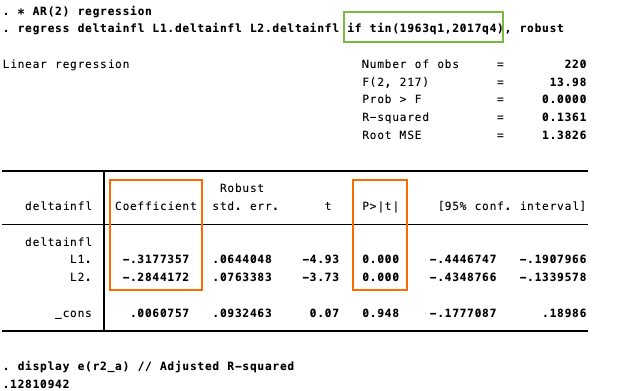
\includegraphics[width=0.9\linewidth]{pictures/(c-ii)AR2} \end{flushleft}
\end{frame}

\begin{frame}{Q(c-iii-I)}
\protect\hypertarget{qc-iii-i}{}
\begin{flushleft}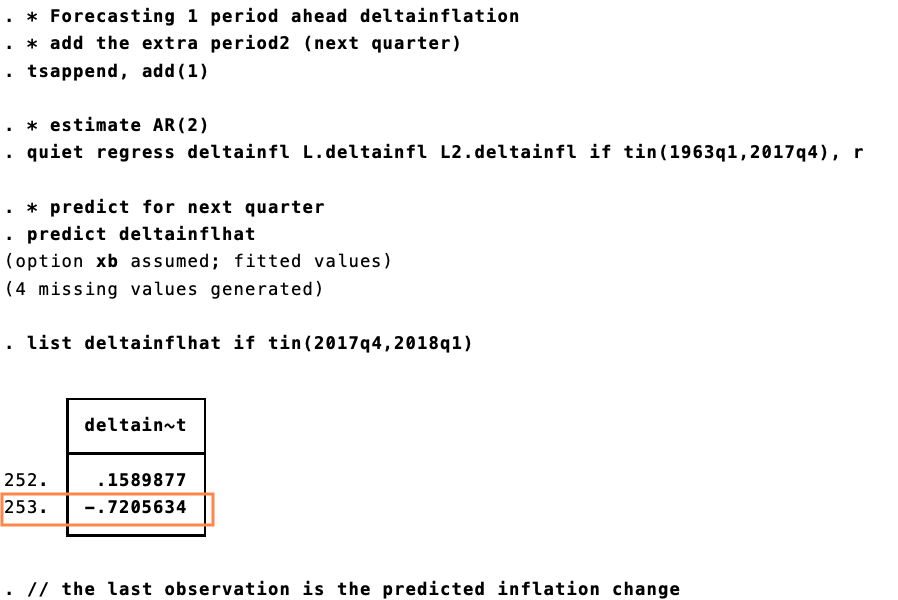
\includegraphics[width=0.9\linewidth]{pictures/(ciii)forecasting} \end{flushleft}
\end{frame}

\begin{frame}{Q(c-iii-II)
\footnotesize \protect\hyperlink{Plot-forecasting-A}{(\textgreater\textgreater back(c-iii))}
\normalsize }
\protect\hypertarget{Plot-forecasting}{}
\begin{flushleft}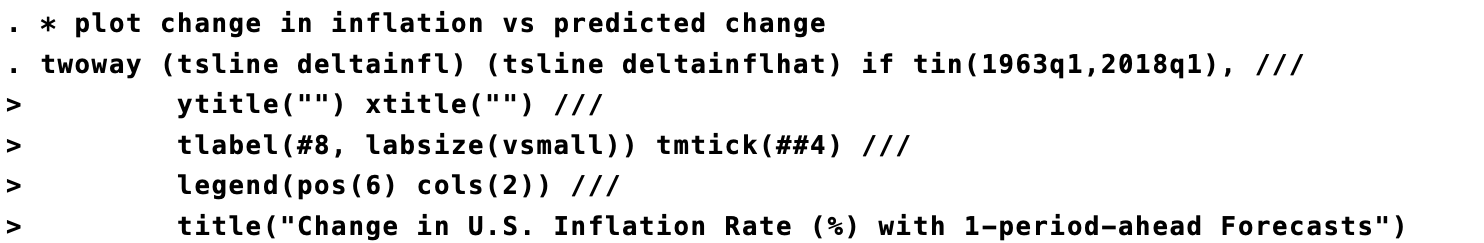
\includegraphics[width=0.9\linewidth]{pictures/(c-iii)Plot-forecasting} \end{flushleft}
\end{frame}

\begin{frame}{Q(d-i)
\footnotesize \protect\hyperlink{ADFtest-stochastic-A}{(\textgreater\textgreater back(d-i))}
\normalsize }
\protect\hypertarget{ADFtest-stochastic}{}
\begin{flushleft}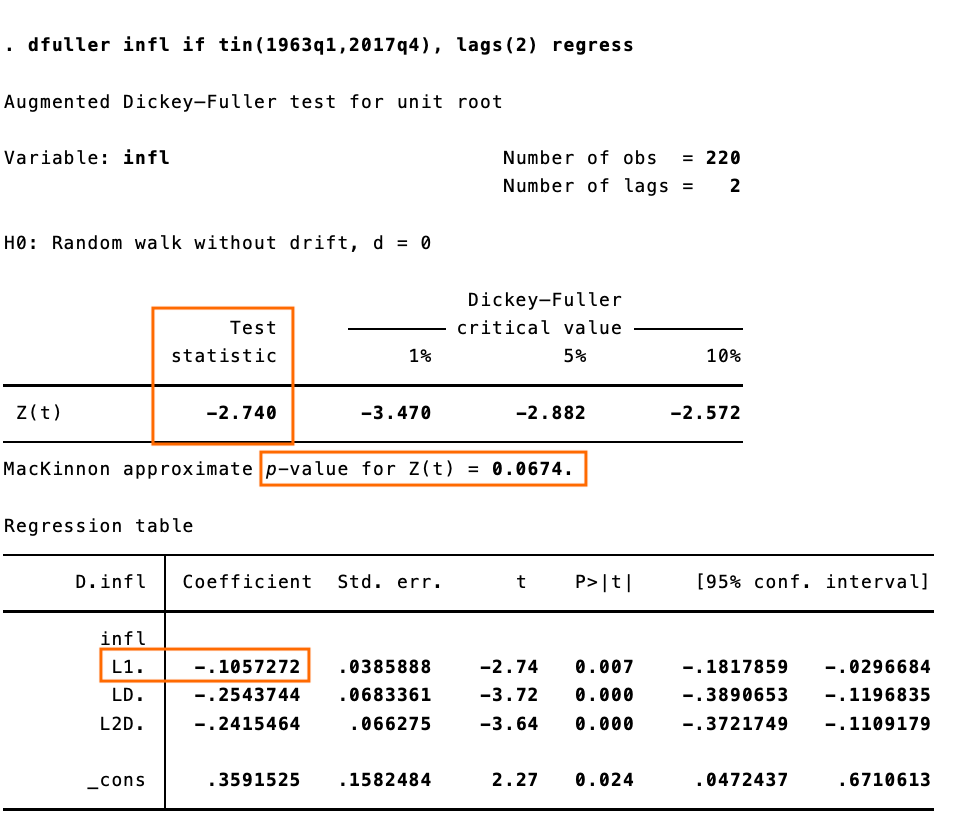
\includegraphics[width=0.7\linewidth]{pictures/(d-i)ADFtest-stochastic} \end{flushleft}
\end{frame}

\begin{frame}{Q(d-ii)
\footnotesize \protect\hyperlink{ADFtest-deterministic-A}{(\textgreater\textgreater back(d-ii))}
\normalsize }
\protect\hypertarget{ADFtest-deterministic}{}
\begin{flushleft}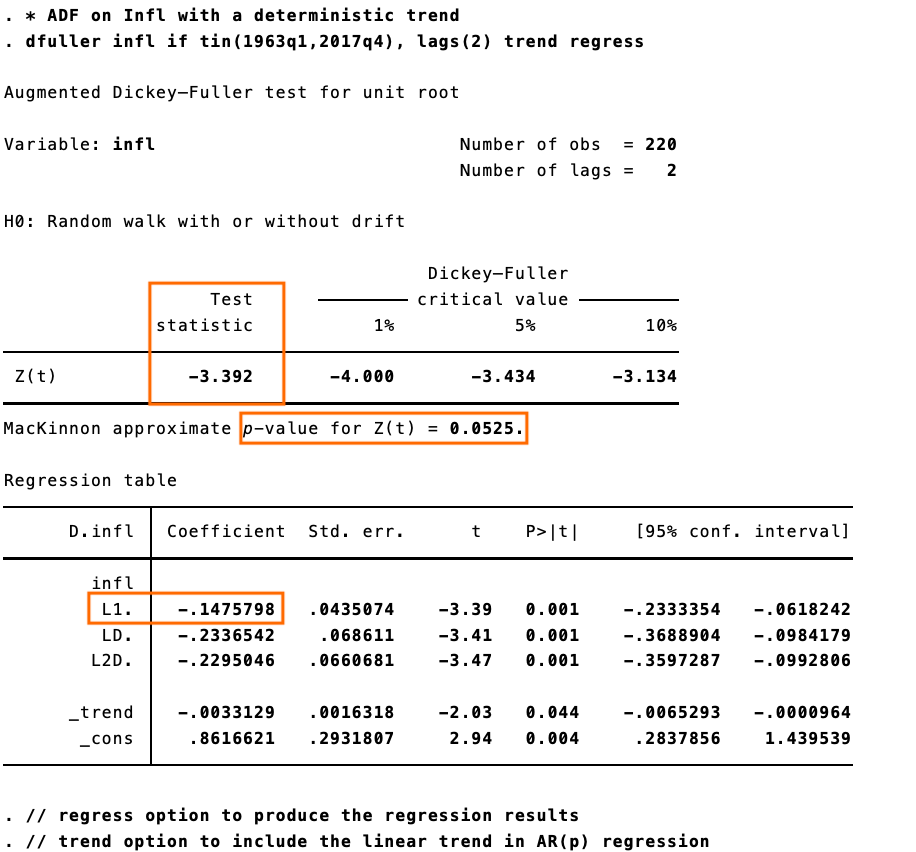
\includegraphics[width=0.7\linewidth]{pictures/(d-ii)ADFtest-deterministic} \end{flushleft}
\end{frame}

\end{document}
